\documentclass[fleqn,11pt,openany]{book}

% These two need to be set before including scirun style package
\title{SCIRun Visualization Basics}
\author{Ayla Khan, David Weinstein}

% INCLUDE SCI STYLE DOCUMENT
\usepackage{scirun}

\begin{document}

%% starting from SCIRun Doc wiki
%% http://software.sci.utah.edu/SCIRunDocs/index.php/CIBC:Documentation:SCIRun:Tutorial:BioPSE


% CREATE TITLE PAGE --------------------------------------------------
\maketitle

% CHAPTERS ---------------------------------------------------------------

\chapter{SCIRun Overview} \label{overview}

\begin{introduction}
This tutorial demonstrates how to build a simple SCIRun dataflow network.
\end{introduction}

\section{Software requirements}

\subsection{SCIRun  \SCIRunVersion}

Download SCIRun version \SCIRunVersion and the SCIRunData archive from the
\href{http://www.scirun.org}{SCI software portal}.
Make sure to update to the most up-to-date build available, which will include
the latest bug fixes.

The easiest way to get started with SCIRun is to download and install
a binary version for Windows or Mac OS X.
Sources are available for Linux, however this option is recommended
only for advanced Linux users.

Unpack the SCIRunData archive in a convenient location.
Recall from the User Guide that the path to data can be set using the
\textenvvar{SCIRUN\_DATA} environment variable or by setting
\textenvvar{SCIRUN\_DATA} in the \emph{.scirunrc} file.

%%\subsection{SCIRun SVN}

\chapter{Simple Dataflow Network}

\begin{introduction}
Scope: \hyperref[readdata]{Read Data File} - \hyperref[slice]{Slice} -
\hyperref[visualize]{Visualize} - \hyperref[bbox]{Bounding Box} - \hyperref[isosurface]{Isosurface}
\end{introduction}

\section{Slice Field}

\subsection{Read Data File}\label{readdata}

Read and manipulate a structured mesh dataset.
Create a \textbf{ReadField} module by going to the Modules menu and selecting
the module from the \textbf{SCIRun DataIO} submenu.
Recall from the User Guide that a module can be located in the Modules
menu tree by entering all or part of it's name in the
\textbf{Show Module} text input.

Navigate to the SCIRunData directory and select the dataset \emph{volume/engine.nhdr}.

\begin{figure}[H]
\scalebox{0.3}{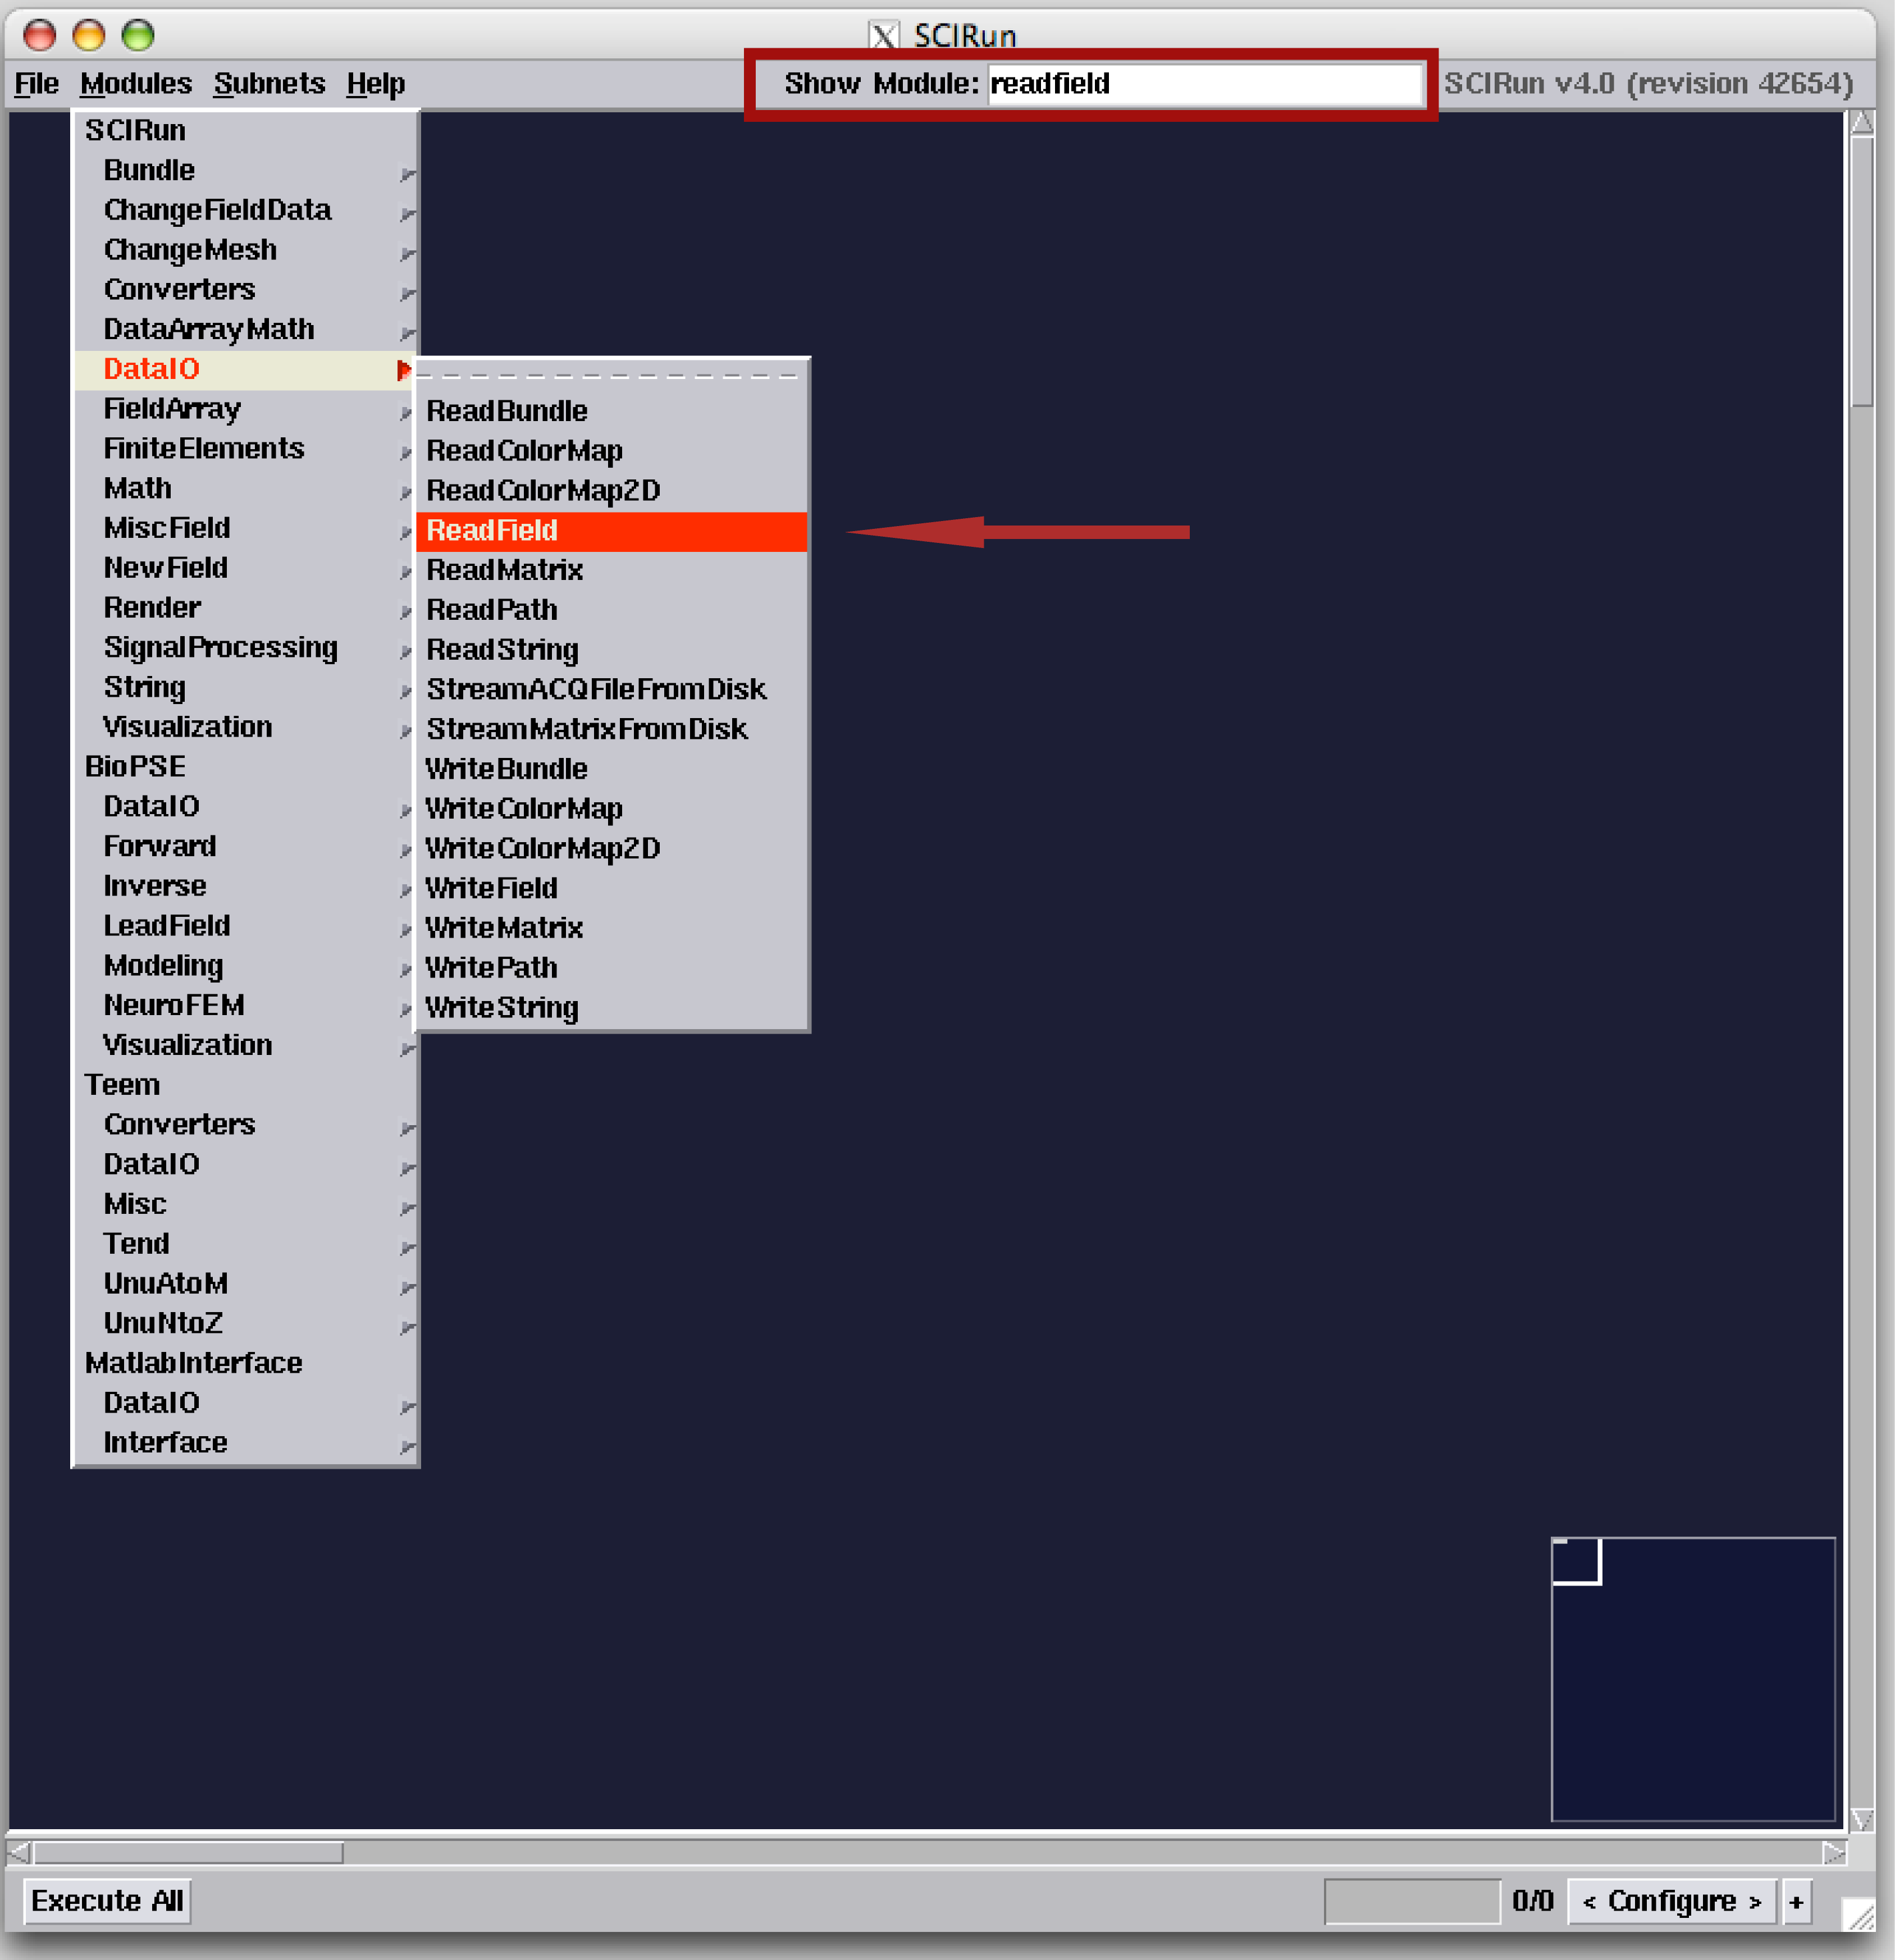
\includegraphics{BasicTutorial_figures/readfield.png}}
\caption{Locate ReadField module.}
\label{fig:readfield}
\end{figure}

\begin{figure}[H]
\scalebox{0.3}{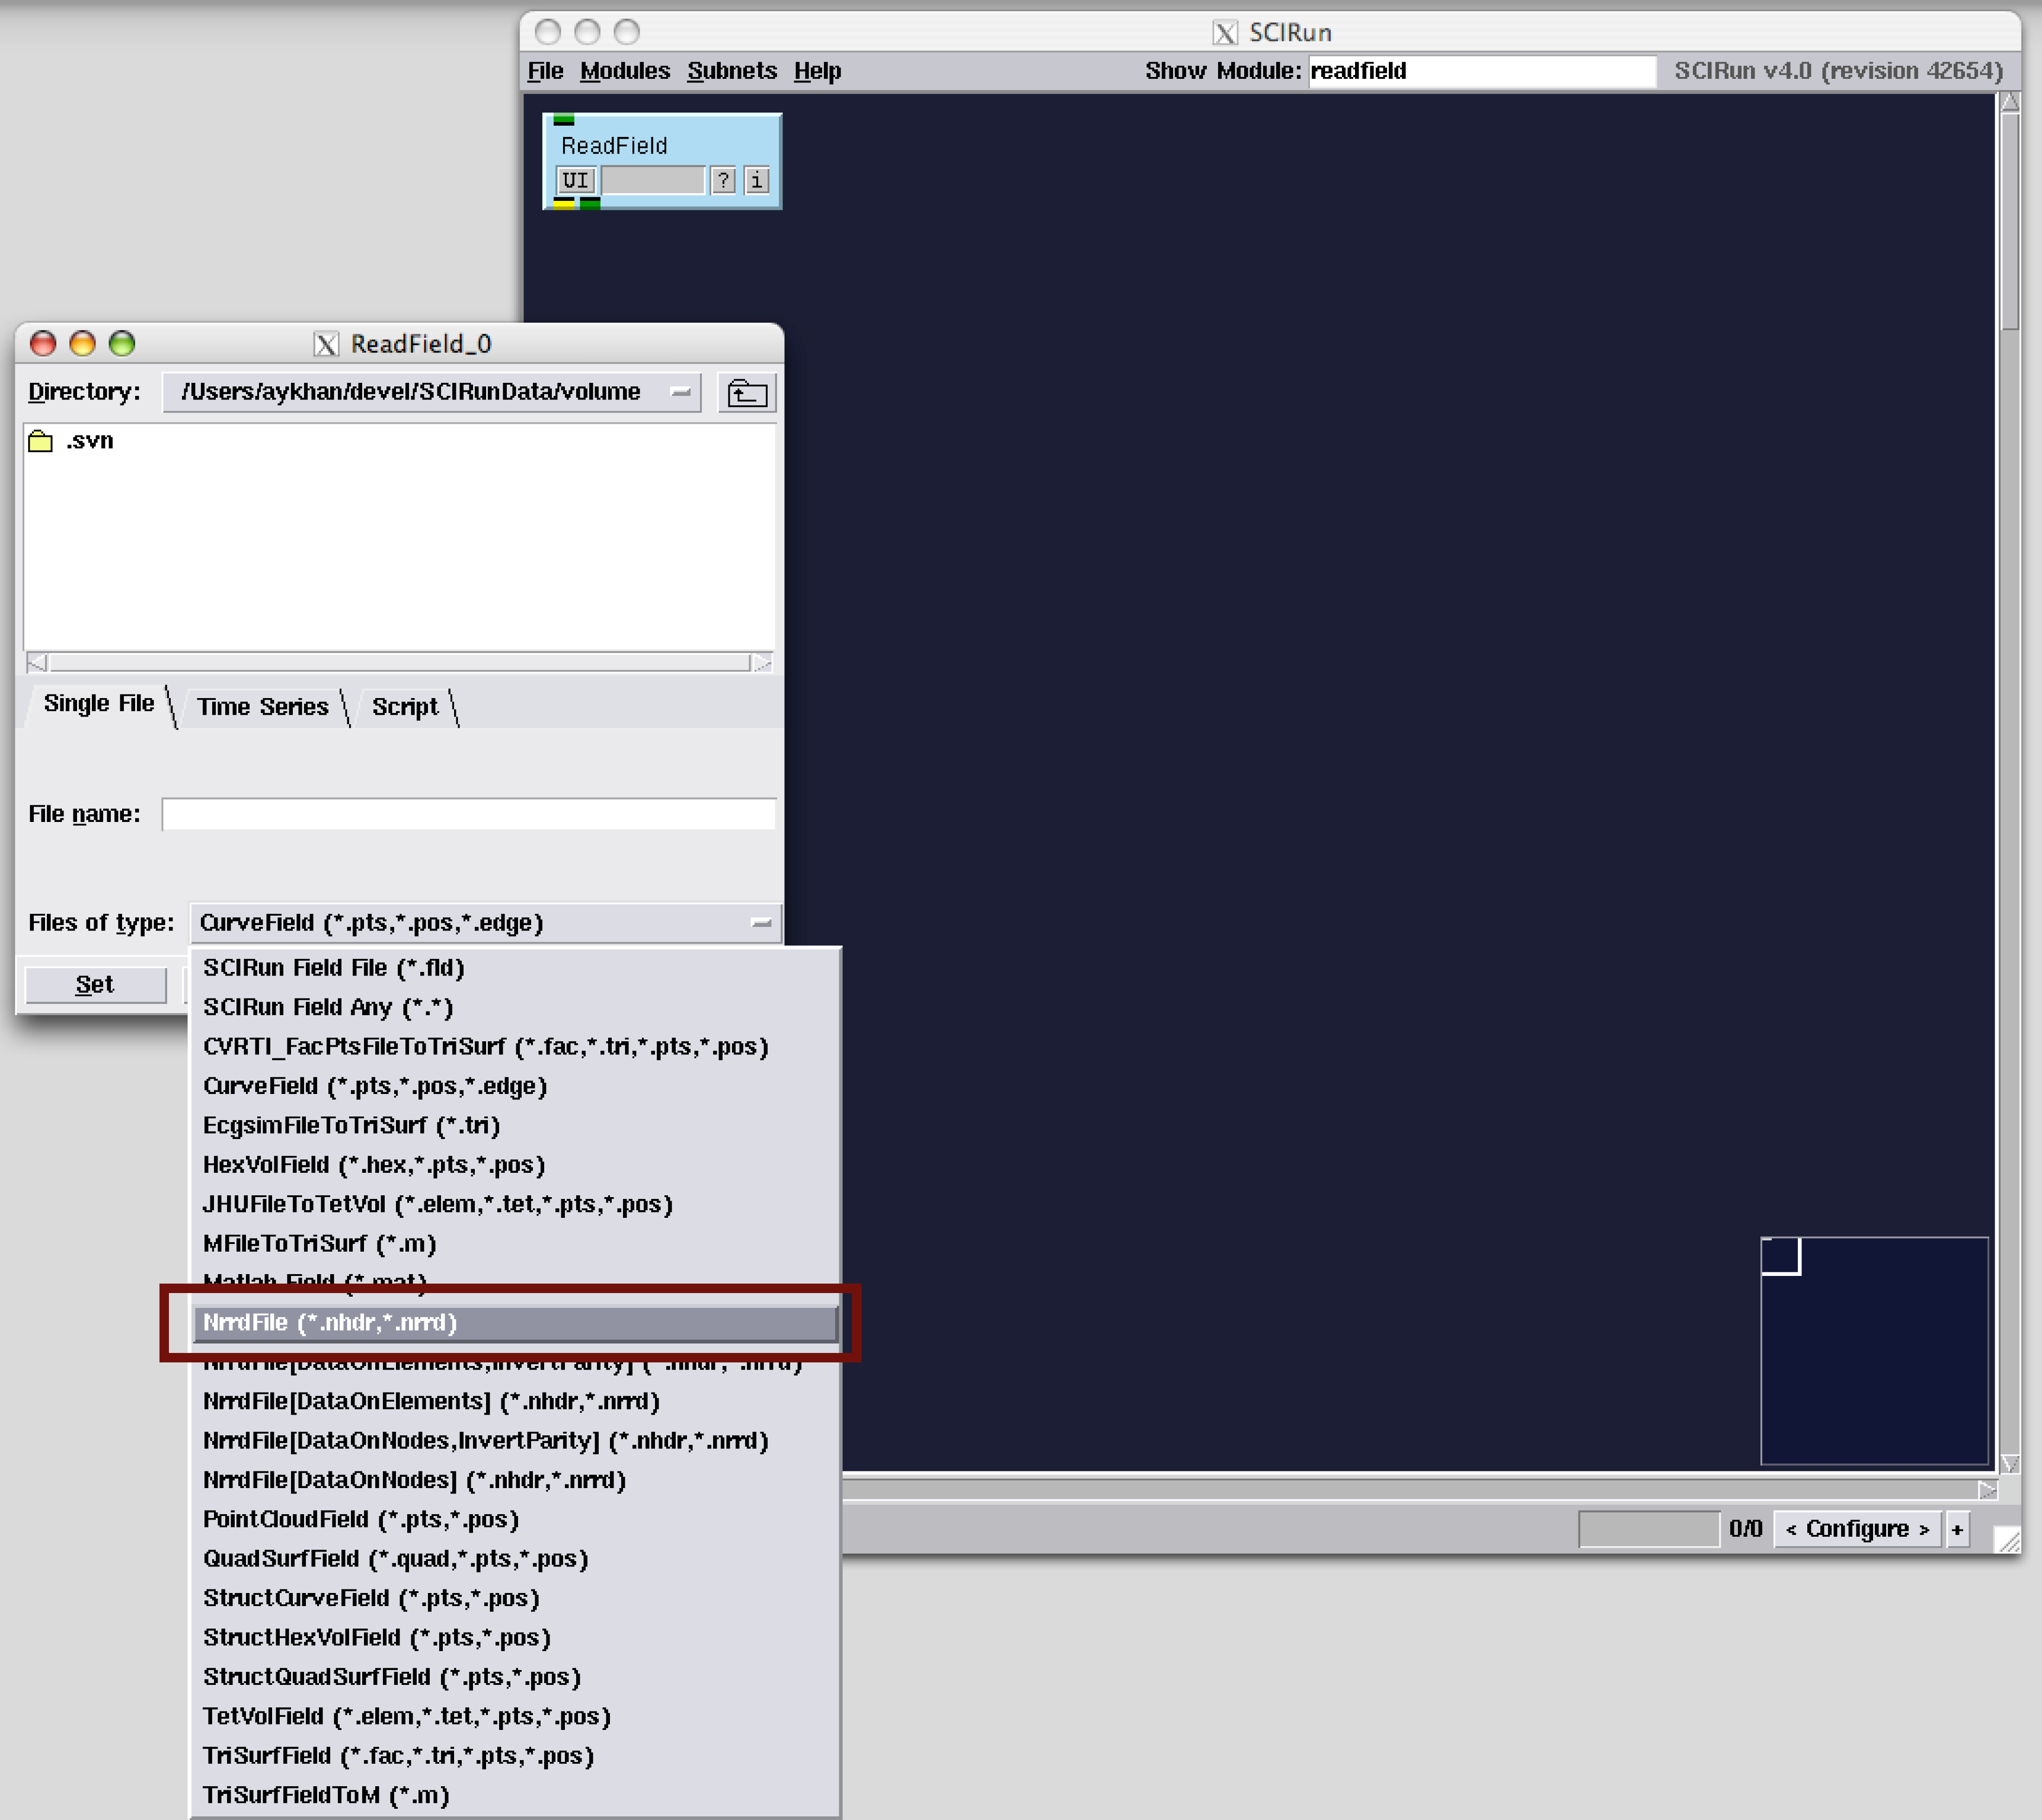
\includegraphics{BasicTutorial_figures/readfield_selecttype.png}}
\caption{ReadField can be used to read many data file formats.}
\label{fig:readfieldtype}
\end{figure}

\subsection{Slice Field}\label{slice}

Slice the engine field by node index along a given axis by instantiating the module
\textbf{GetSlicesFromStructuredFieldByIndices} and connecting it to \textbf{ReadField}.

\begin{figure}[H]
\scalebox{0.3}{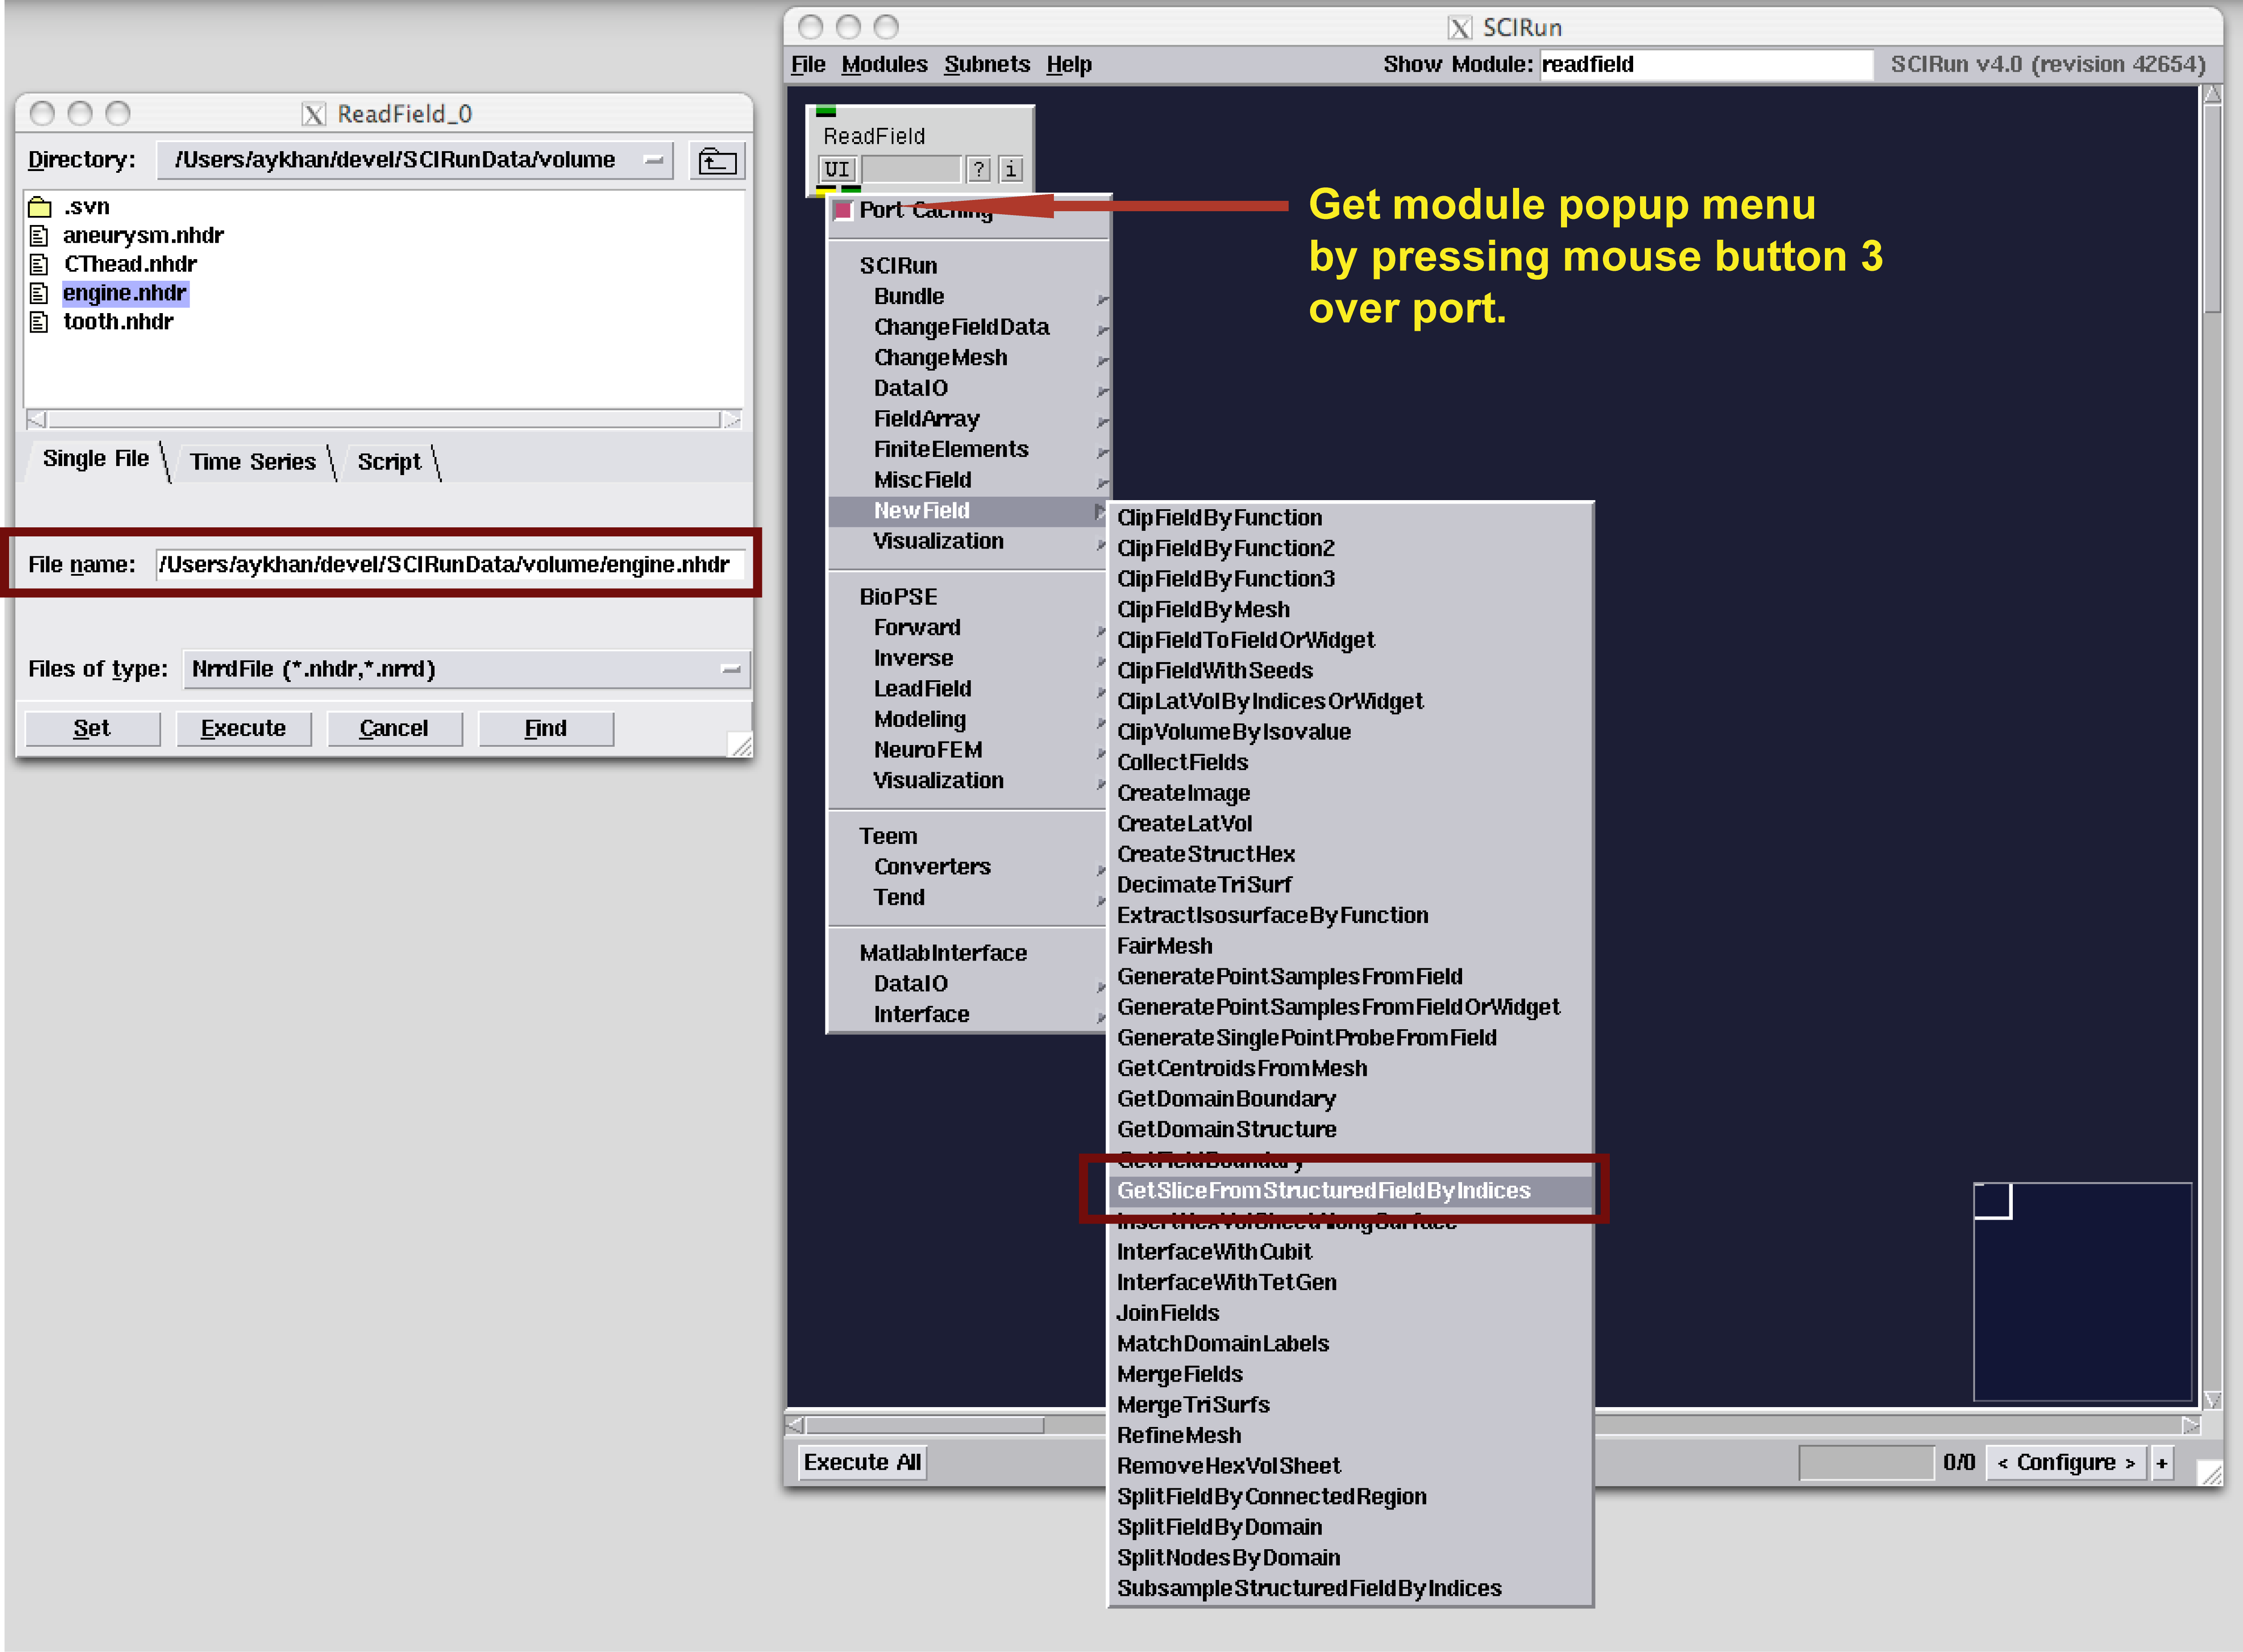
\includegraphics{BasicTutorial_figures/getslicemodule.png}}
\caption{Using the ReadField Field port's popup menu to instantiate GetSliceFromStructuredFieldByIndices.}
\label{fig:slicemod}
\end{figure}

\subsection{Visualize Field}\label{visualize}

To visualize the field geometry, instantiate module \textbf{ShowField}
in the \textbf{Visualization} category and module \textbf{ViewScene}
in the \textbf{Render} category.
ShowField takes a field as input, and outputs scene-graph geometry.
ViewScene displays the geometry and allows a user to interact with the scene.
Choose colors to apply to the geometry using \textbf{CreateStandardColorMaps}
and \textbf{RescaleColorMaps} modules in textbf{Visualization}.
Execute network and use the sliders in the GetSlicesFromStructuredFieldByIndices UI
to change slice position (see figure \ref{fig:viewscene}).

\begin{figure}[H]
\scalebox{0.3}{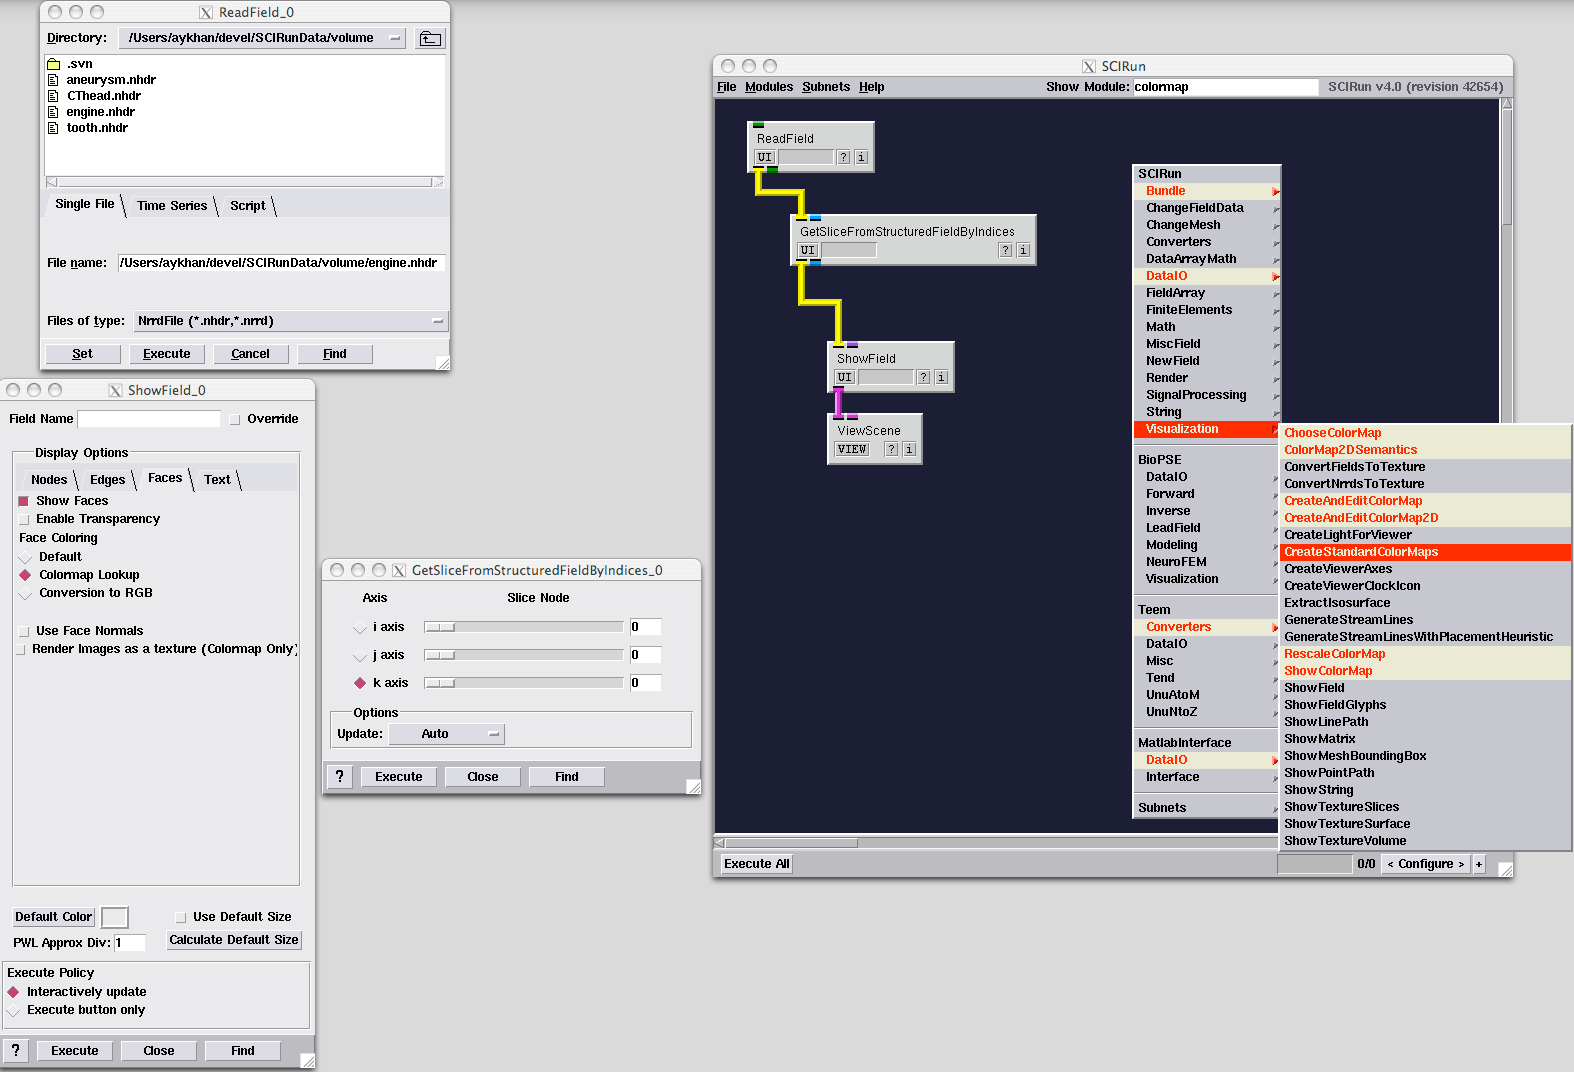
\includegraphics{BasicTutorial_figures/createcolormaps.png}}
\caption{SCIRun provides a useful set of default colormaps.}
\label{fig:colormap}
\end{figure}

\begin{figure}[H]
\scalebox{0.3}{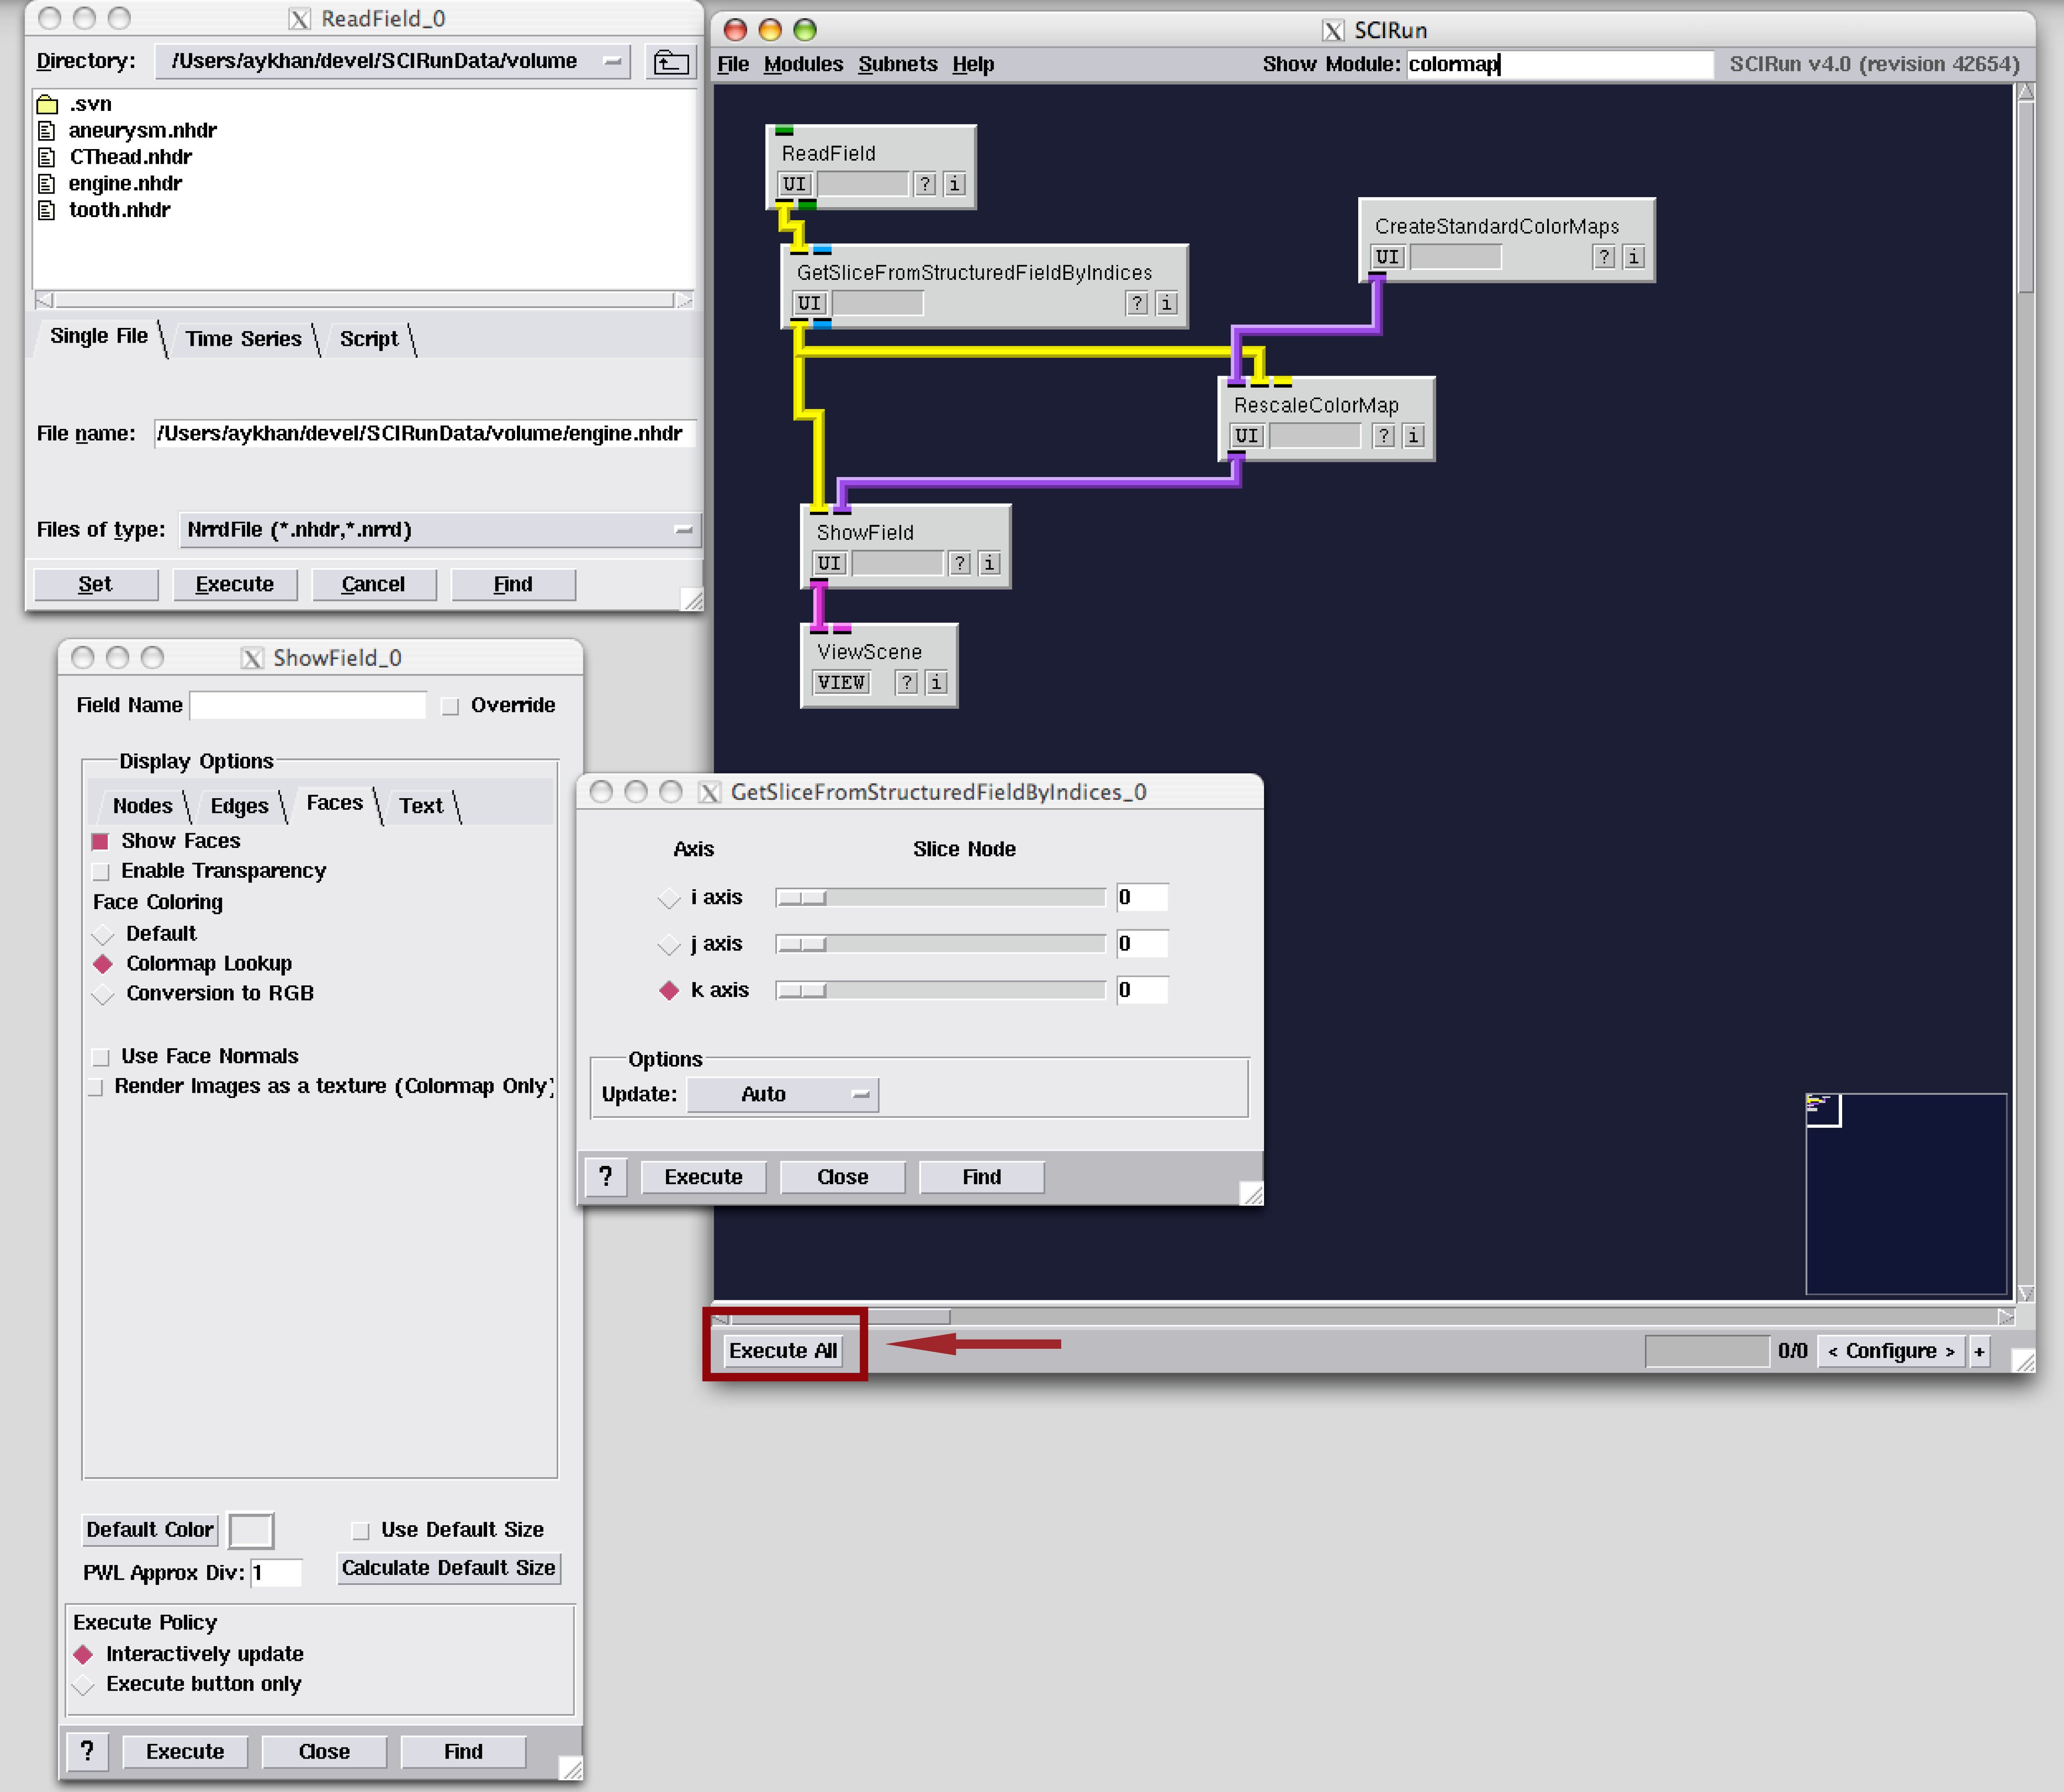
\includegraphics{BasicTutorial_figures/rescalecolormap.png}}
\caption{Rescale colormap to data values.}
\label{fig:rescale}
\end{figure}

\begin{figure}[H]
\scalebox{0.3}{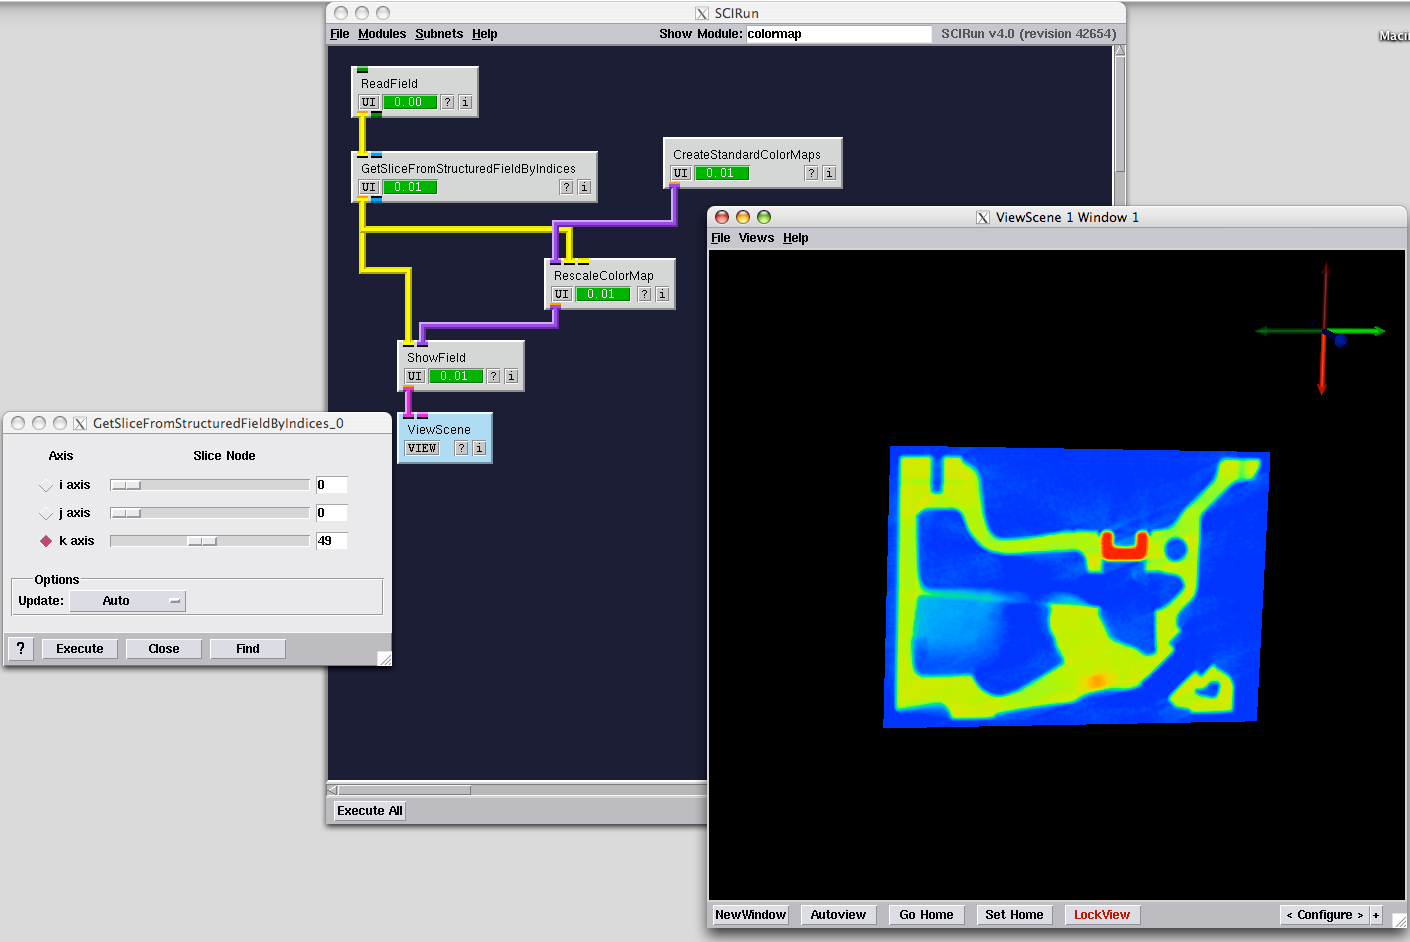
\includegraphics{BasicTutorial_figures/viewscene.png}}
\caption{Visualize the slice field's geometry.}
\label{fig:viewscene}
\end{figure}

\section{Show Bounding Box}\label{bbox}

Add the \textbf{ShowMeshBoundingBox} module and change the number
of lines in cage for each dimension.
Execute the network.

\begin{figure}[H]
\scalebox{0.3}{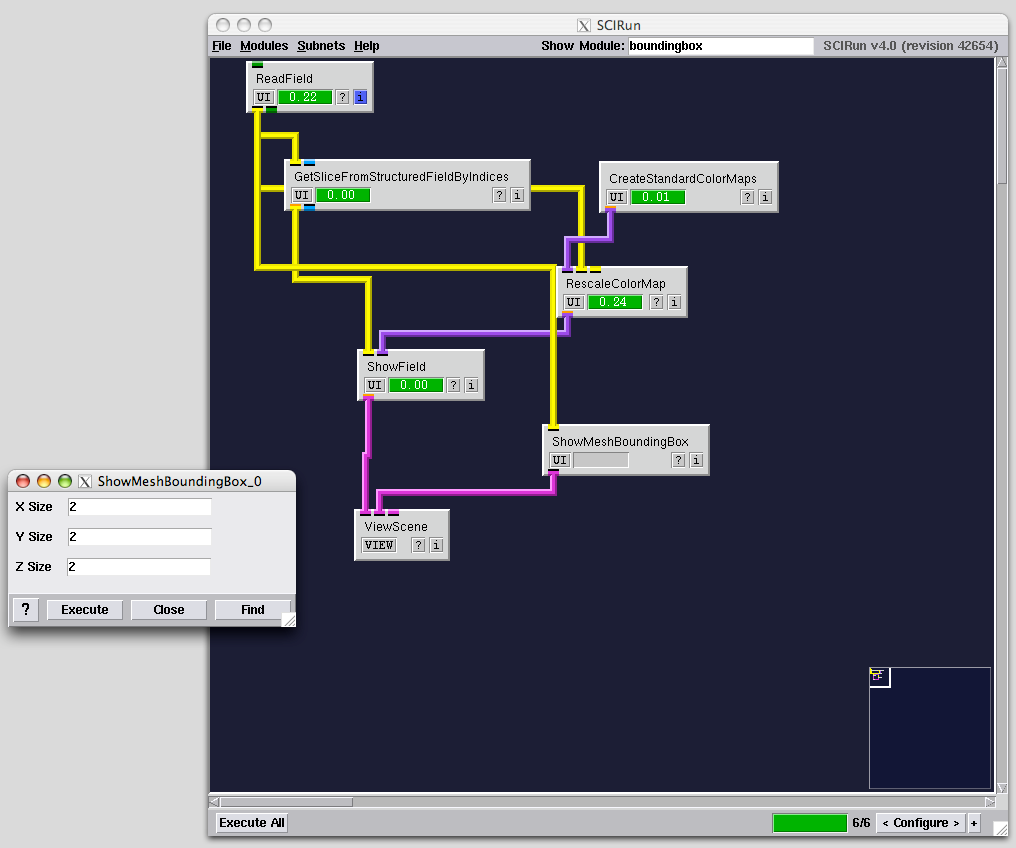
\includegraphics{BasicTutorial_figures/boundingbox.png}}
\caption{Configure bounding box cage.}
\label{fig:addbbox}
\end{figure}

\begin{figure}[H]
\scalebox{0.3}{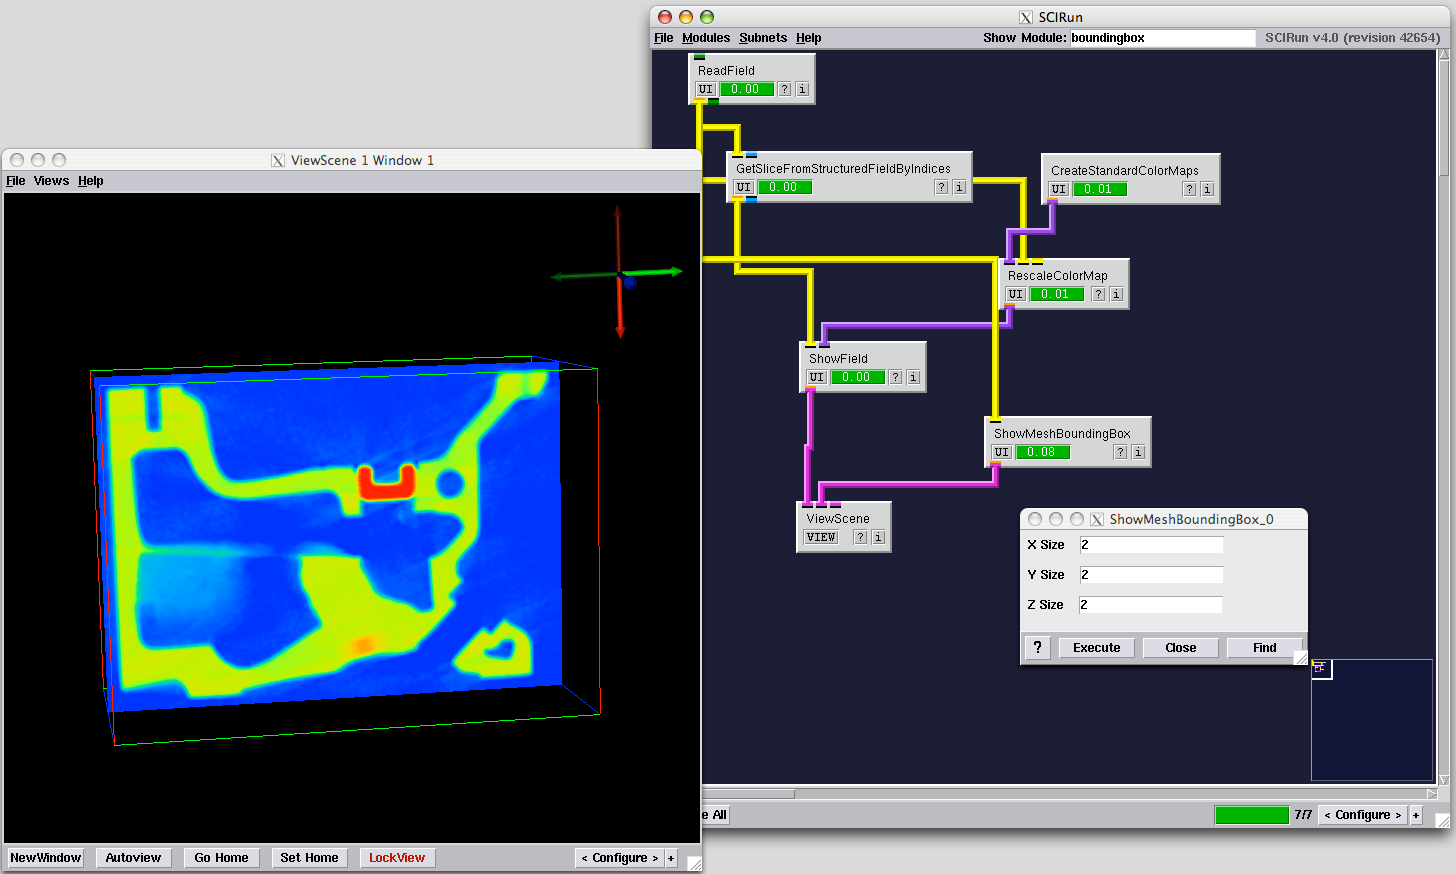
\includegraphics{BasicTutorial_figures/view_boundingbox.png}}
\caption{View the mesh's bounding box.}
\label{fig:viewbbox}
\end{figure}

\section{Isosurface}\label{isosurface}

Construct an isosurface from the field by instantiating and connecting an
\textbf{Visualization} module \textbf{ExtractIsosurface} to ReadField
(figure \ref{fig:extract}).
Color isosurface output geometry by connecting the RescaleColorMap module.
Execute the network and use the slider in the ExtractIsosurface UI to change
the isovalue (see figure \ref{fig:viewisosurf}).

\begin{figure}[H]
\scalebox{0.3}{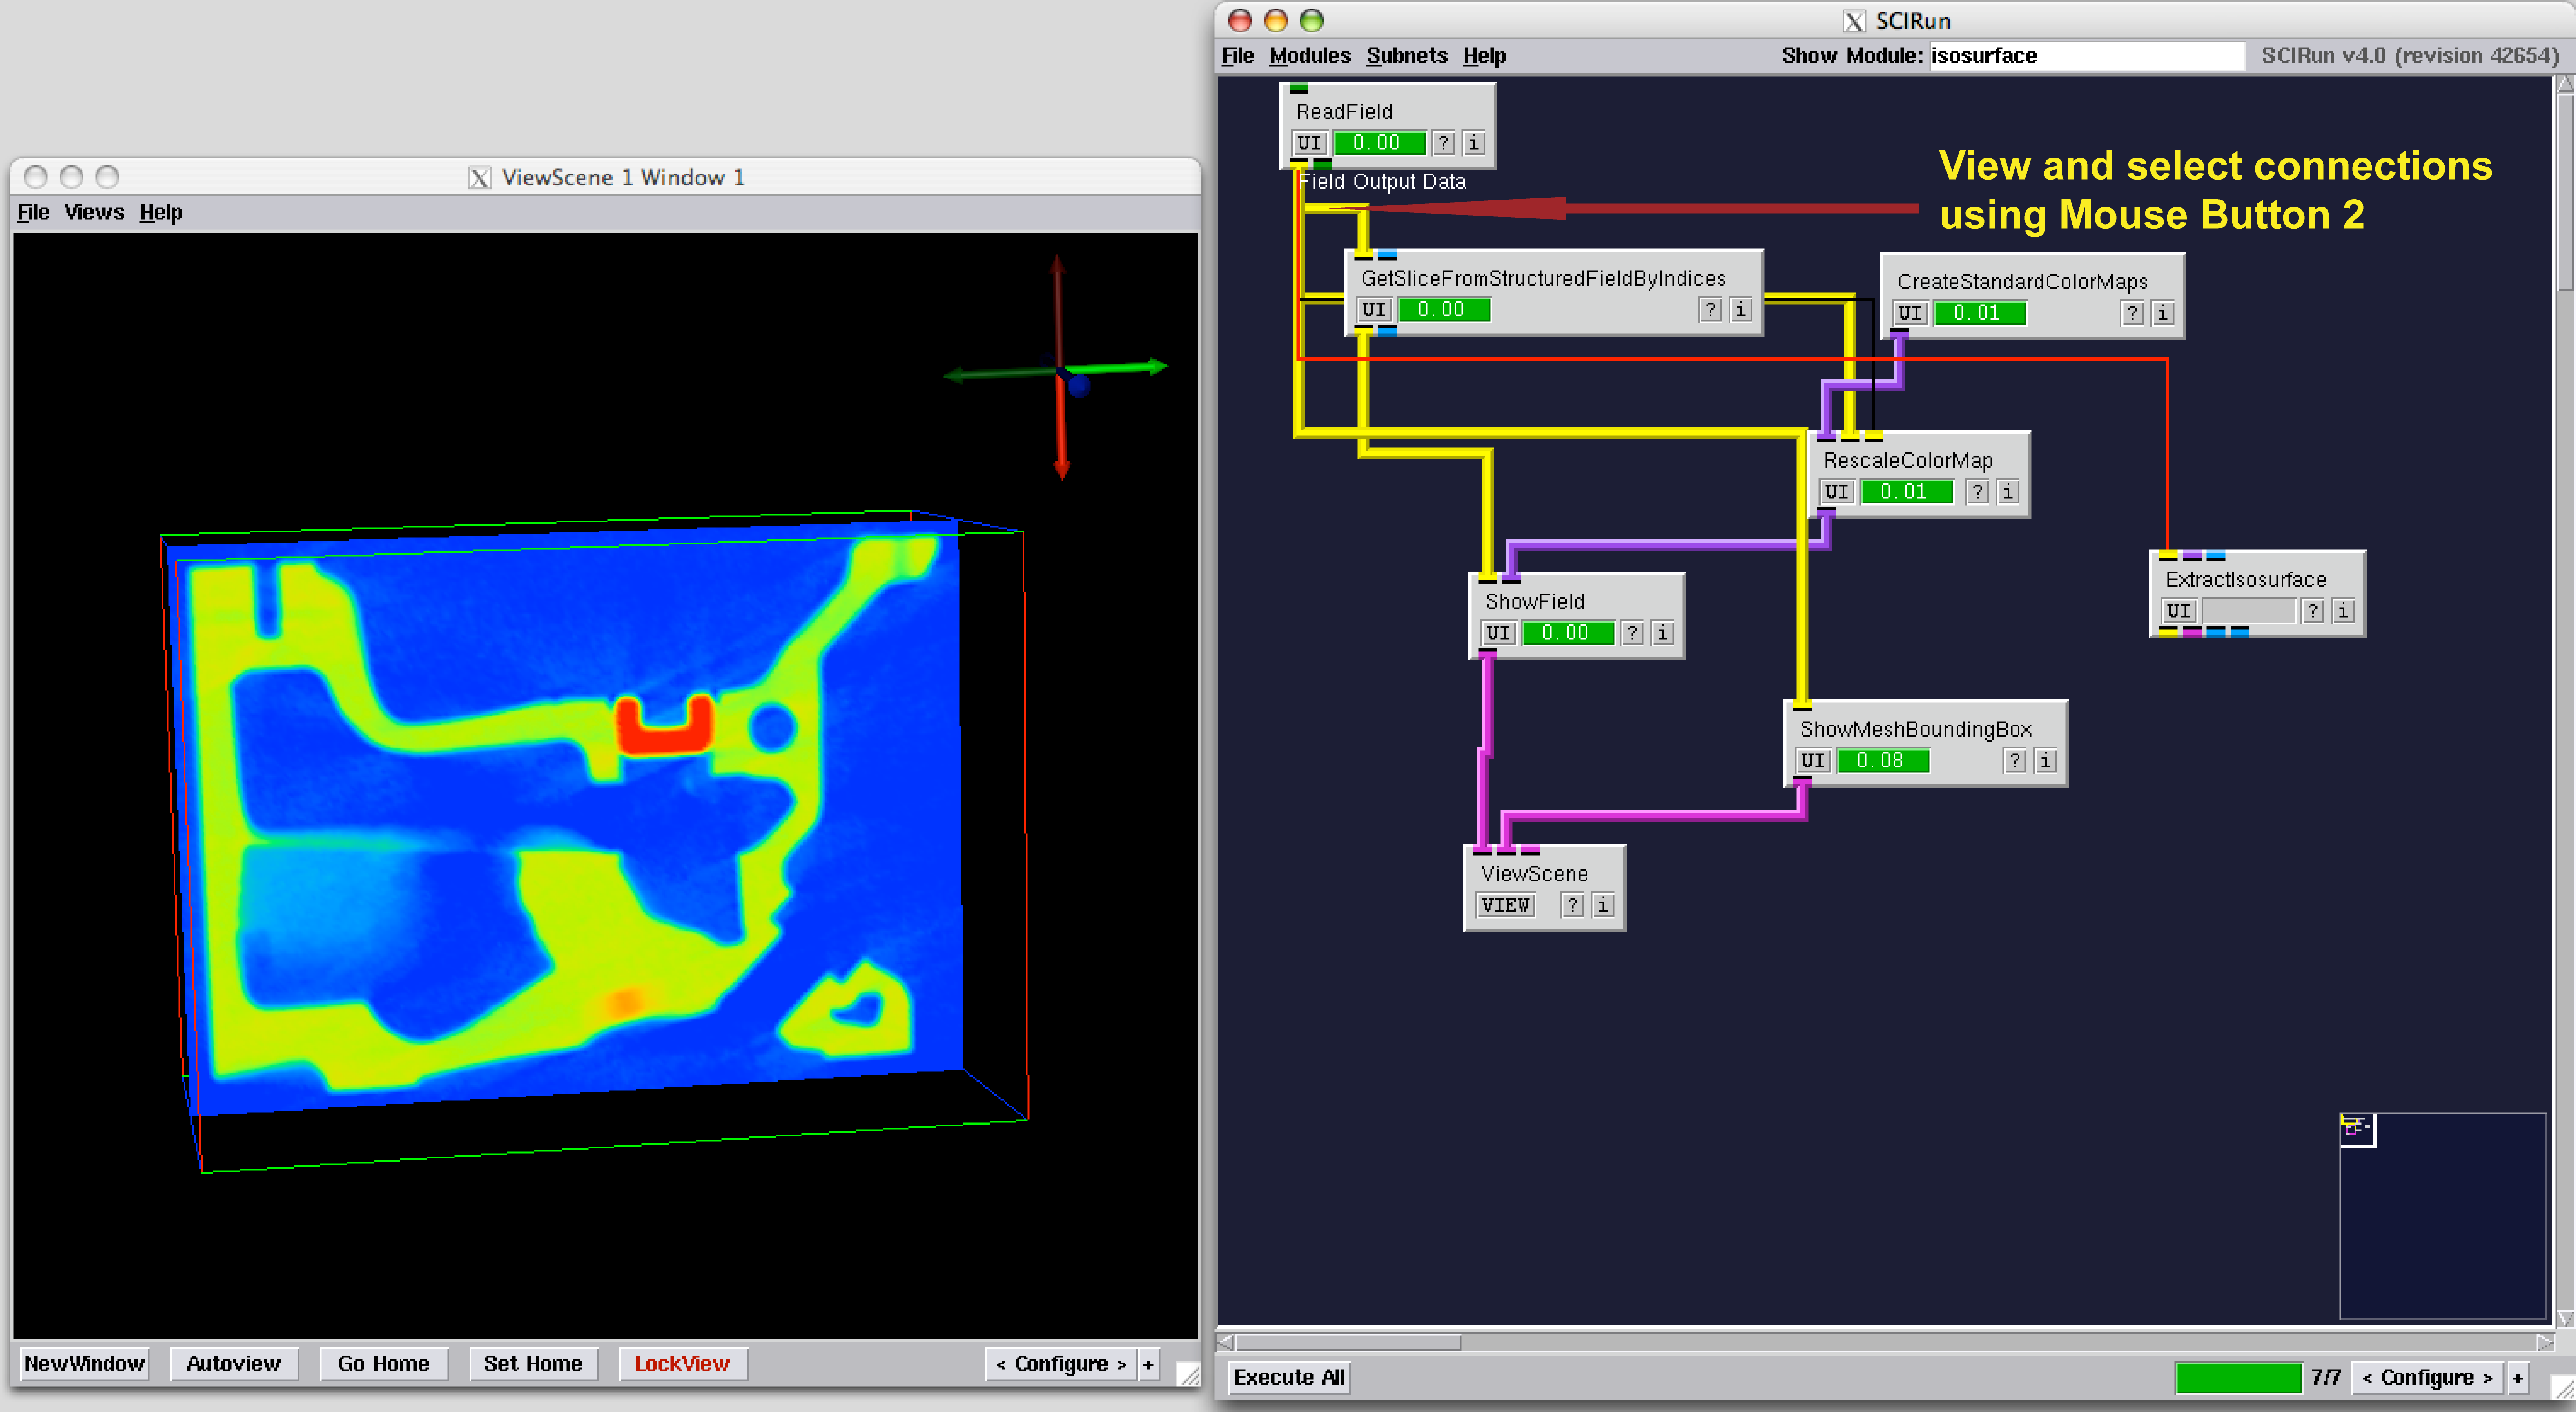
\includegraphics{BasicTutorial_figures/extractisosurface.png}}
\caption{Extract an isosurface from field.}
\label{fig:extract}
\end{figure}

\begin{figure}[H]
\scalebox{0.3}{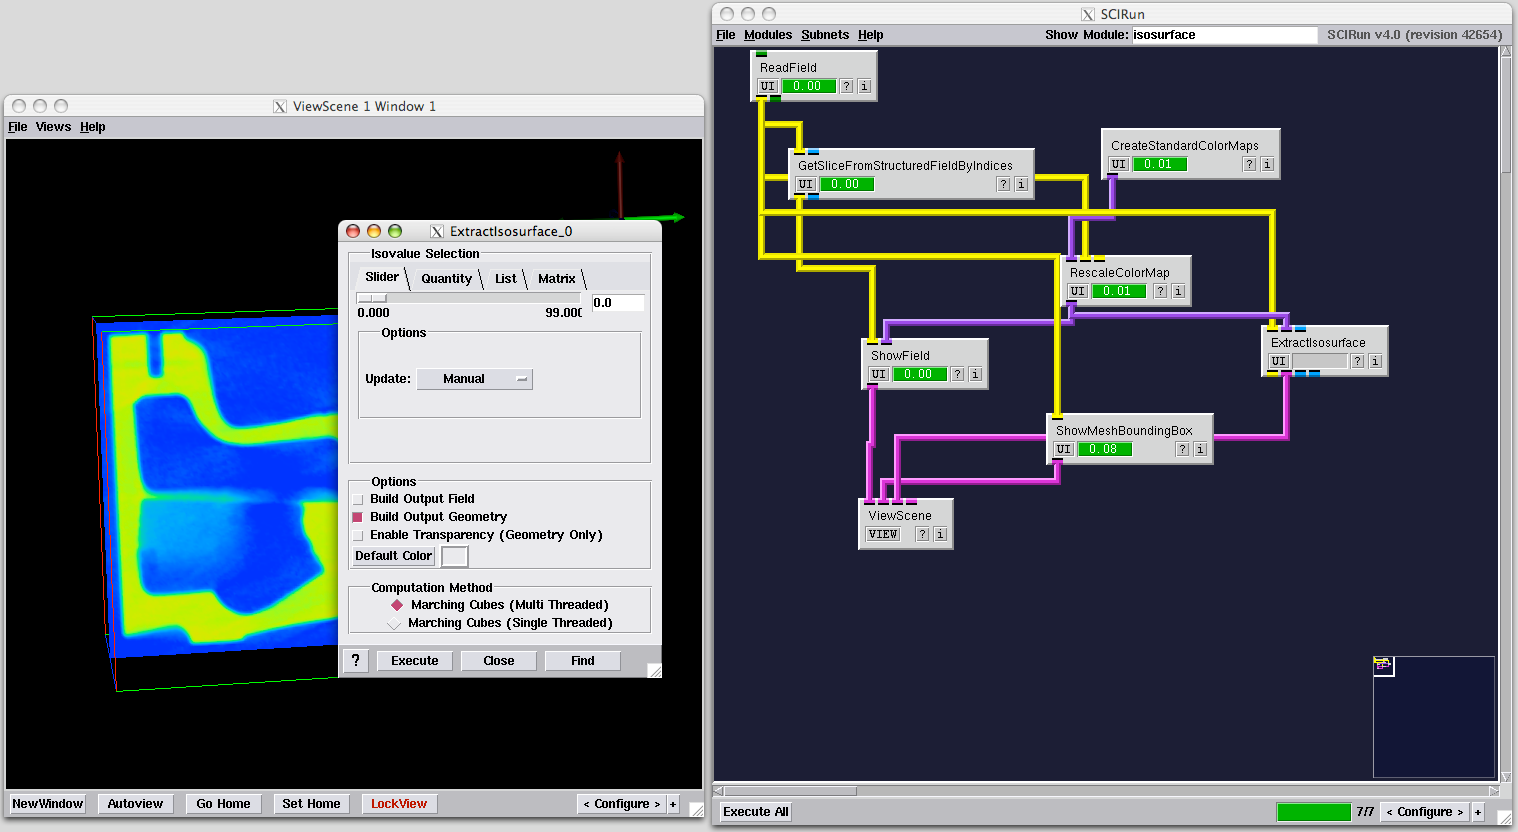
\includegraphics{BasicTutorial_figures/change_isovalue.png}}
\caption{The ExtractIsosurface UI.}
\label{fig:changeisoval}
\end{figure}

\begin{figure}[H]
\scalebox{0.3}{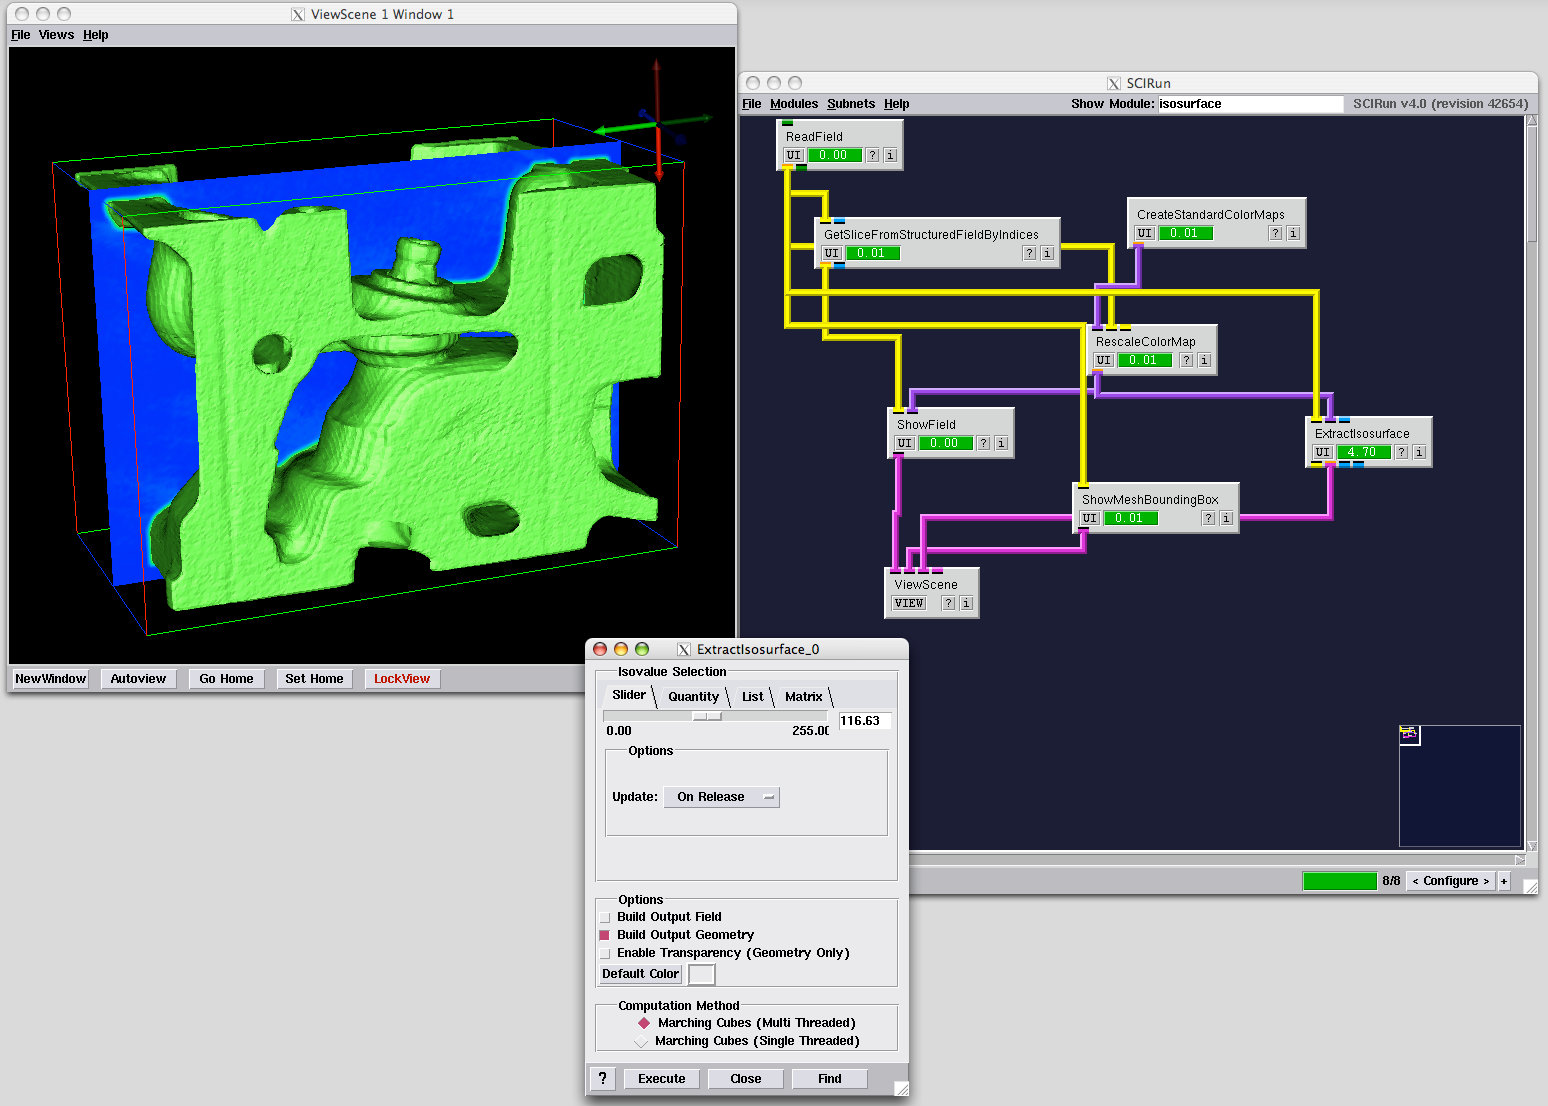
\includegraphics{BasicTutorial_figures/view_isosurface.png}}
\caption{Visualize the isosurface.}
\label{fig:viewisosurf}
\end{figure}

\chapter{Create, Manipulate and Visualize Field}

\begin{introduction}
Scope: \hyperref[createfield]{Generate Lattice Volume} - \hyperref[isosurface2]{Isosurface} -
\hyperref[]{Visualize Geometry}
\end{introduction}

\section{Create Field}\label{createfield}

Create and manipulate a structured mesh type in this exercise.
Start by creating a lattice volume using CreateLatVol module.
Assign data at nodes using CalculateFieldData module.
Connect CalculateFieldData to CreateLatVol and use the expression $RESULT = sqrt(X*X + Y*Y + Z*Z)$ to compute data for each node.

\begin{figure}[H]
\scalebox{0.3}{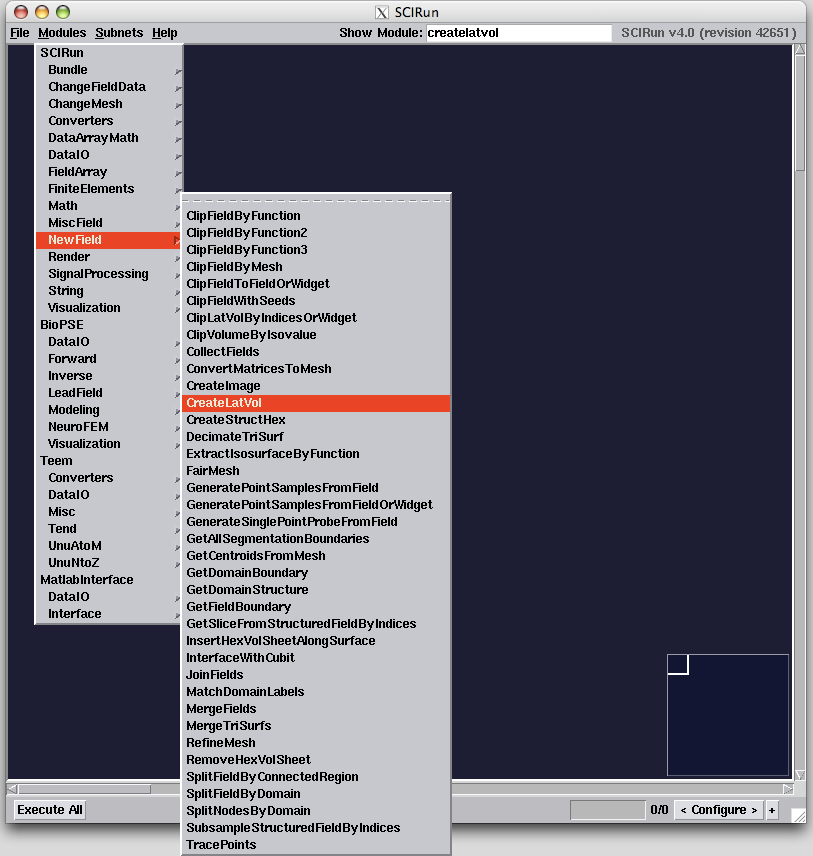
\includegraphics{BasicTutorial_figures/create_newfield.png}}
\caption{Create lattice volume field.}
\label{fig:createnewfield}
\end{figure}

\begin{figure}[H]
\scalebox{0.3}{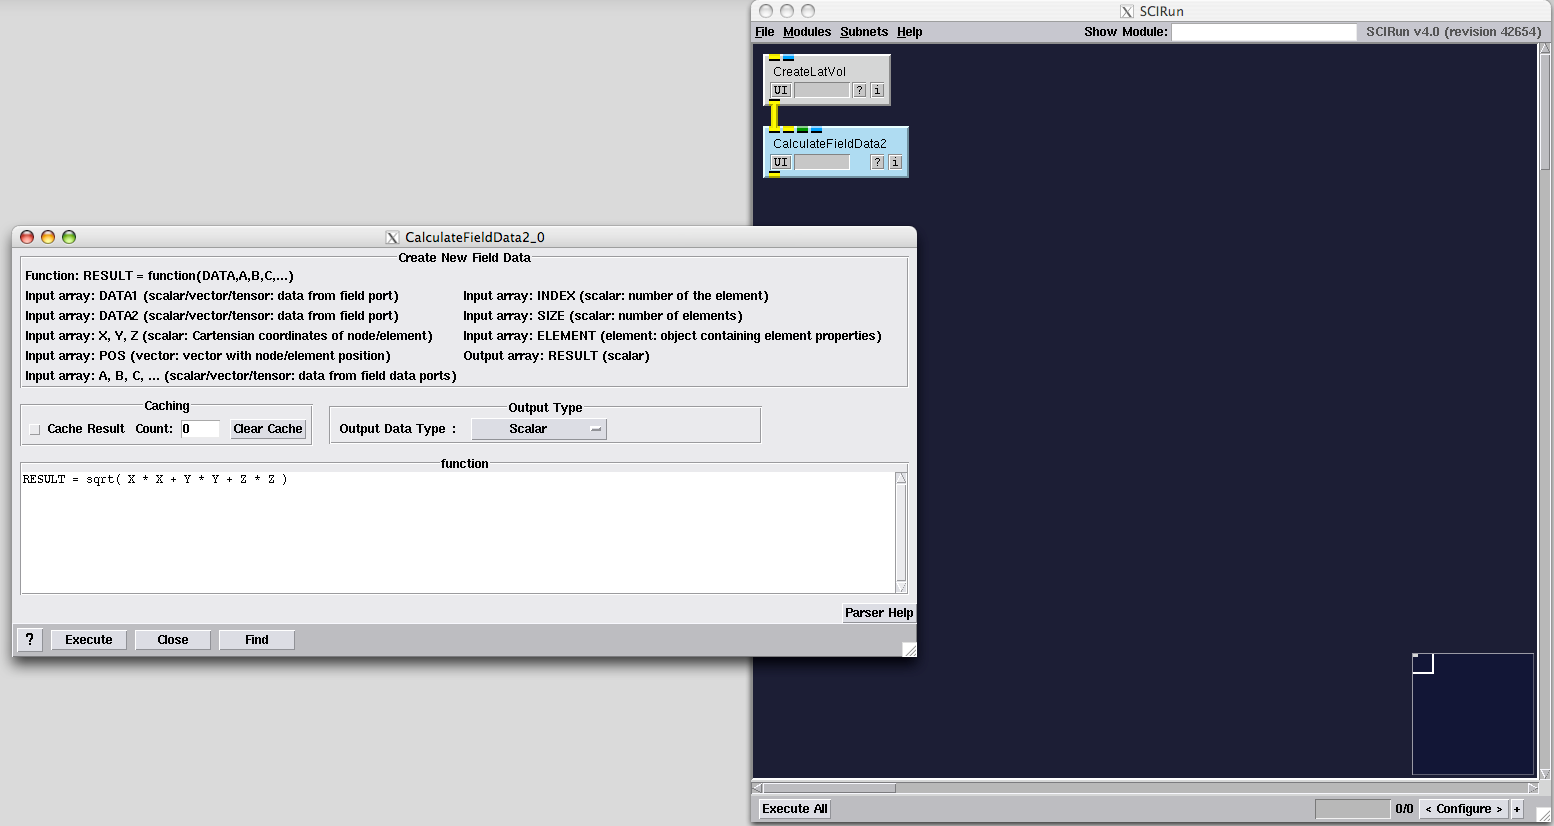
\includegraphics{BasicTutorial_figures/calcfielddata.png}}
\caption{Calculate node data.}
\label{fig:calcfielddata}
\end{figure}

\section{Isosurface}\label{isosurface2}

Generate the isosurface by instantiating and connecting an ExtractIsosurface module to CalculateFieldData.
Complete the network by adding a colormap.
Execute the network and show 4x4x4 mesh bounding box as in section \ref{bbox}.

\begin{figure}[H]
\scalebox{0.3}{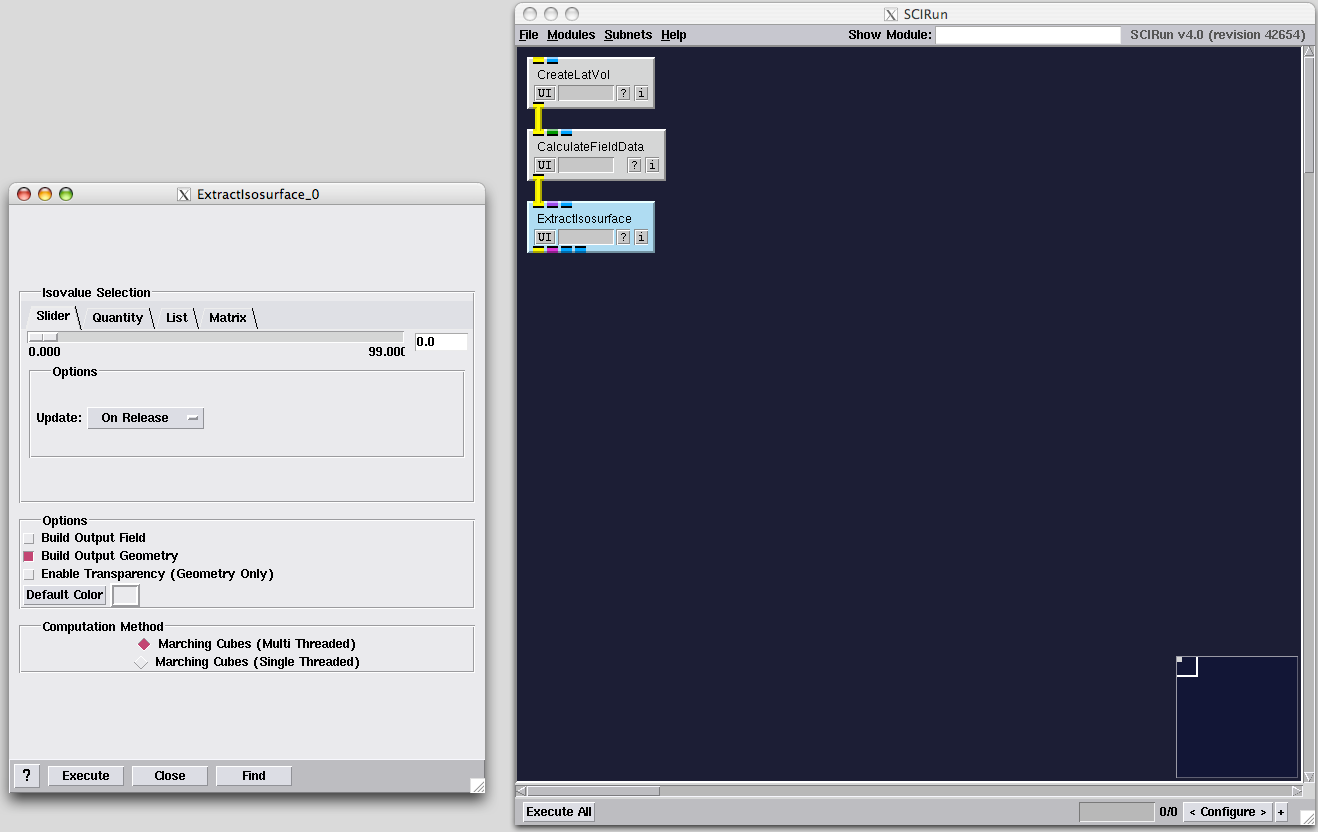
\includegraphics{BasicTutorial_figures/extractisosurface2.png}}
\caption{Extract an isosurface from the field data.}
\label{fig:extractisosurf2}
\end{figure}

\begin{figure}[H]
\scalebox{0.3}{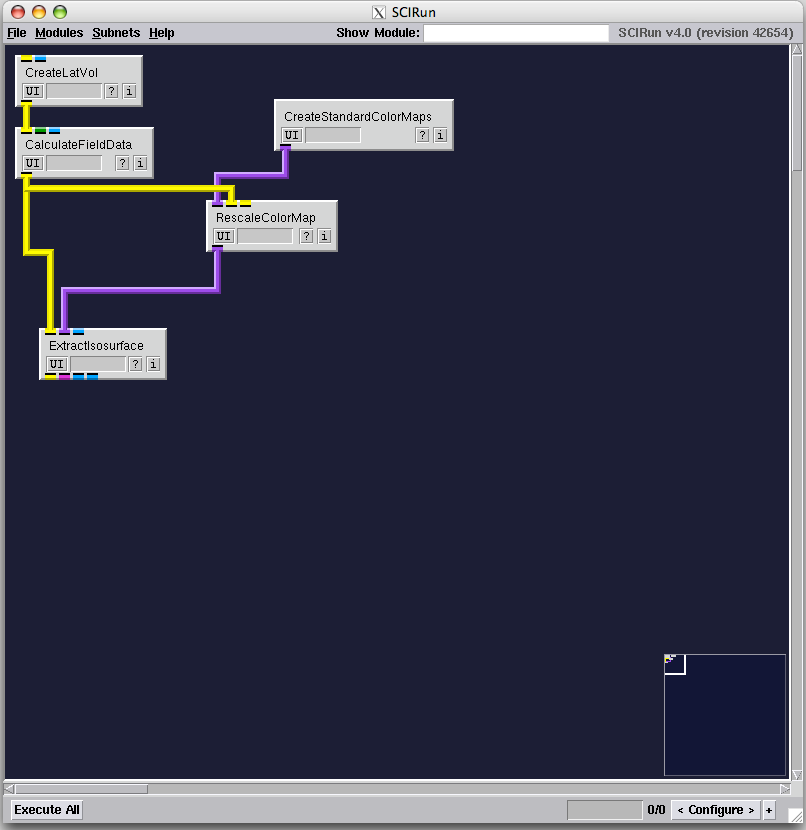
\includegraphics{BasicTutorial_figures/connect_colormaps.png}}
\caption{Map color to the isovalue.}
\label{fig:conncolormap}
\end{figure}

\begin{figure}[H]
\scalebox{0.2}{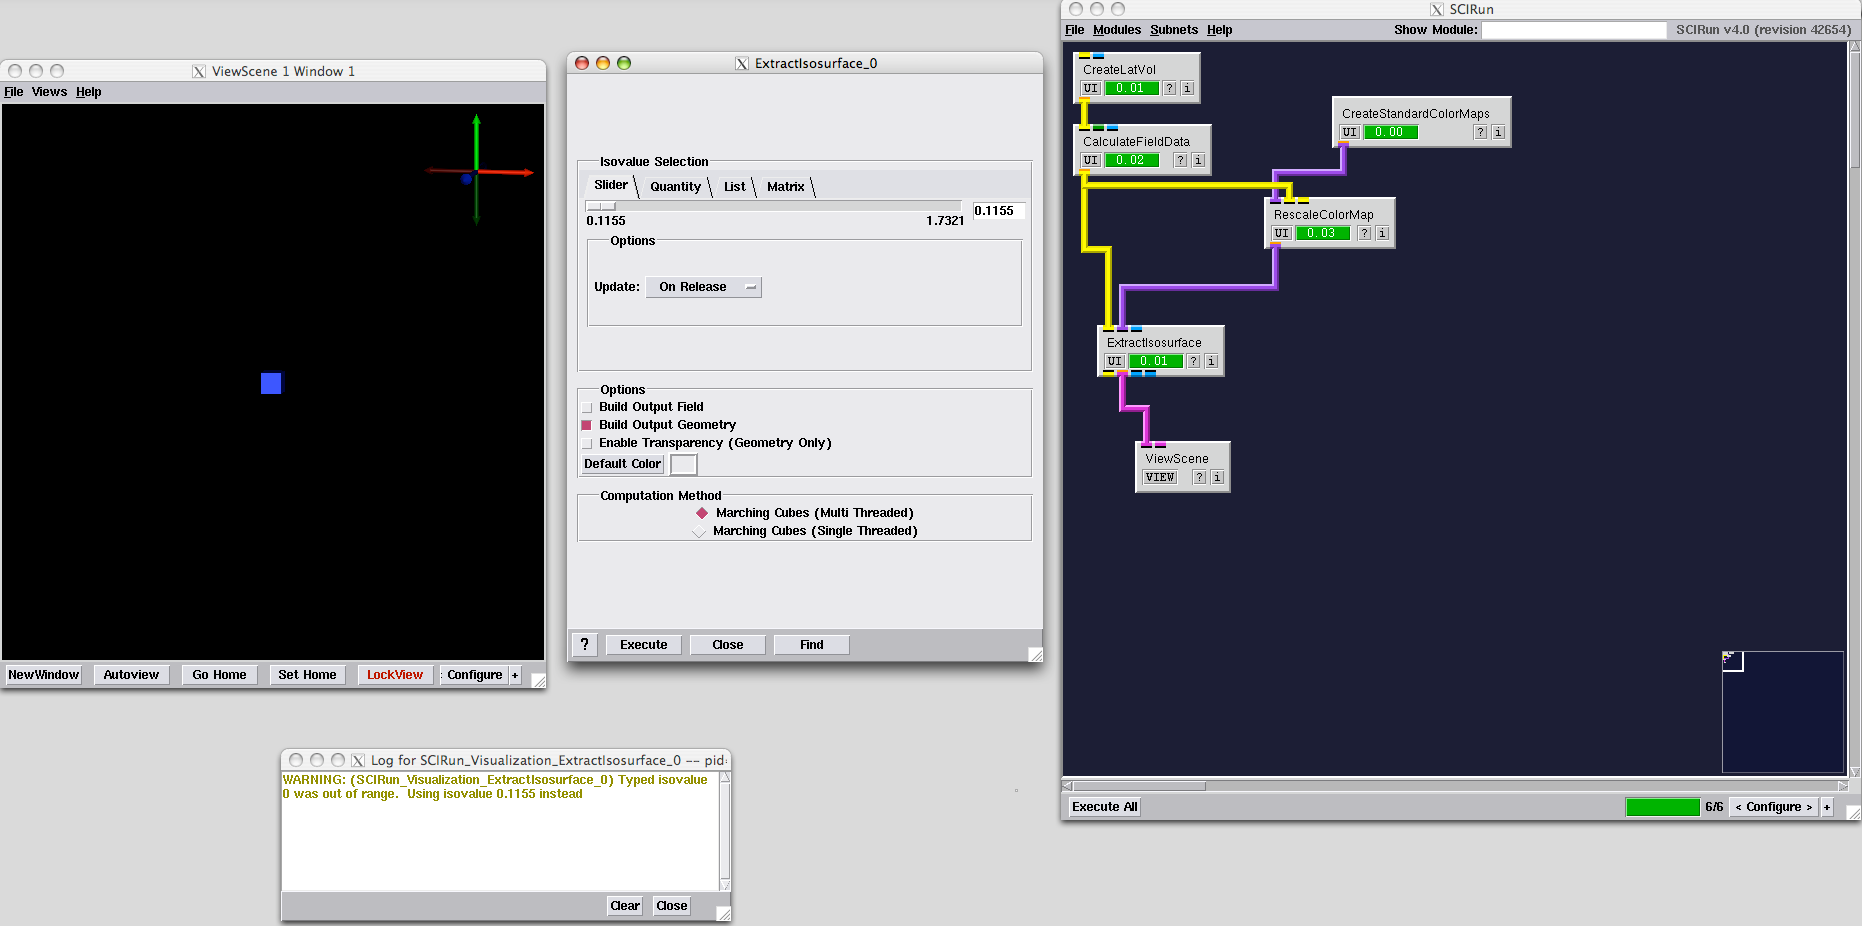
\includegraphics{BasicTutorial_figures/view_defaultisosurface.png}}
\caption{Change the default isovalue.}
\label{fig:viewdefaultisosurf}
\end{figure}

\begin{figure}[H]
\scalebox{0.3}{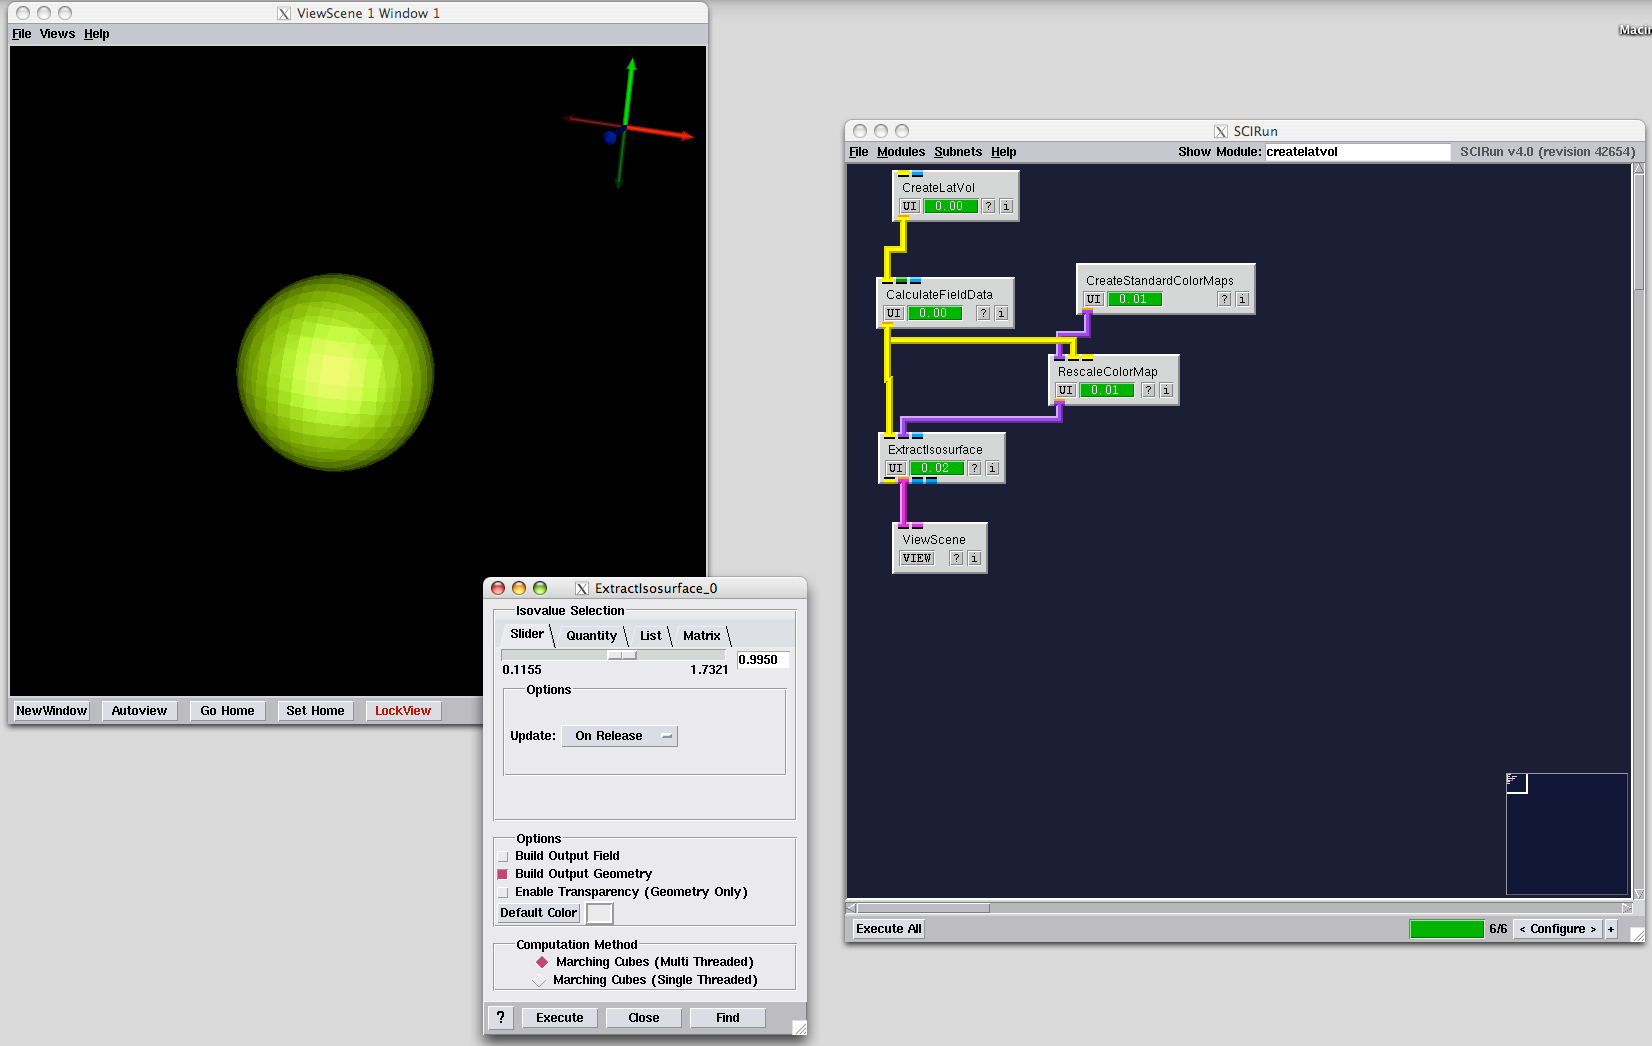
\includegraphics{BasicTutorial_figures/change_isovalue2.png}}
\caption{Visualize the isosurface.}
\label{fig:changeisoval2}
\end{figure}

\begin{figure}[H]
\scalebox{0.3}{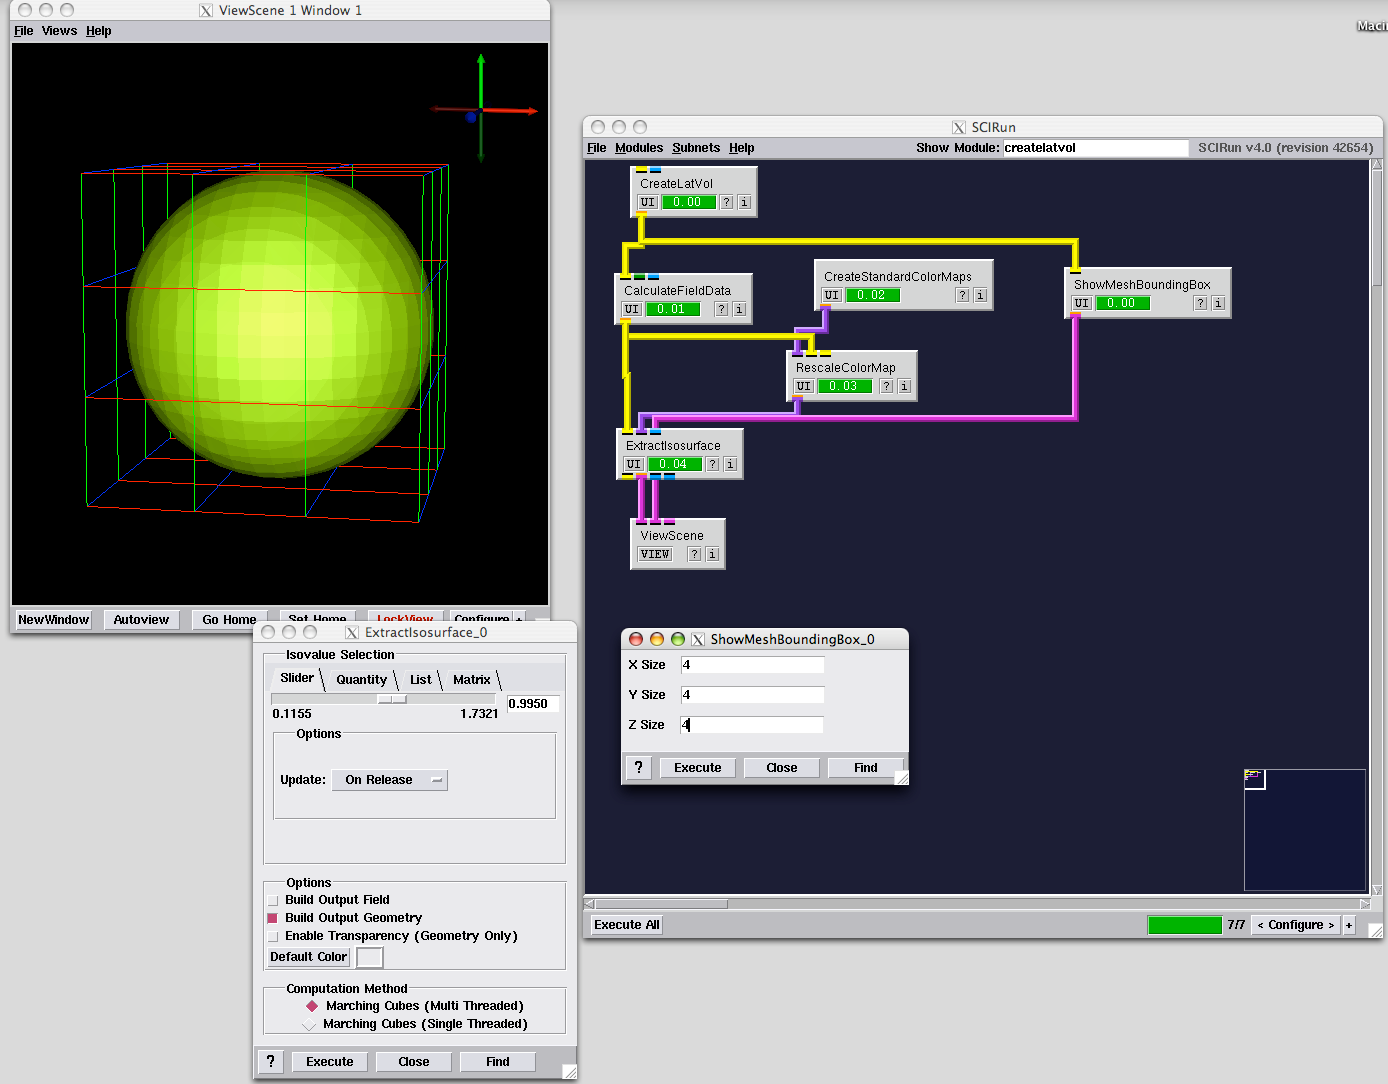
\includegraphics{BasicTutorial_figures/add_boundingbox.png}}
\caption{Show the field's bounding box.}
\label{fig:addbbox2}
\end{figure}

\section{Slice Field}\label{slice2}

%%TODO: should add blurb about disabling modules and add image
%%
%% Postpone until SCIRun 5 due to disabled modules bugs.
Extend the functionality of this network by slicing the field using GetSliceFromStructuredFieldByIndices as in section \ref{slice}.

\begin{figure}[H]
\scalebox{0.3}{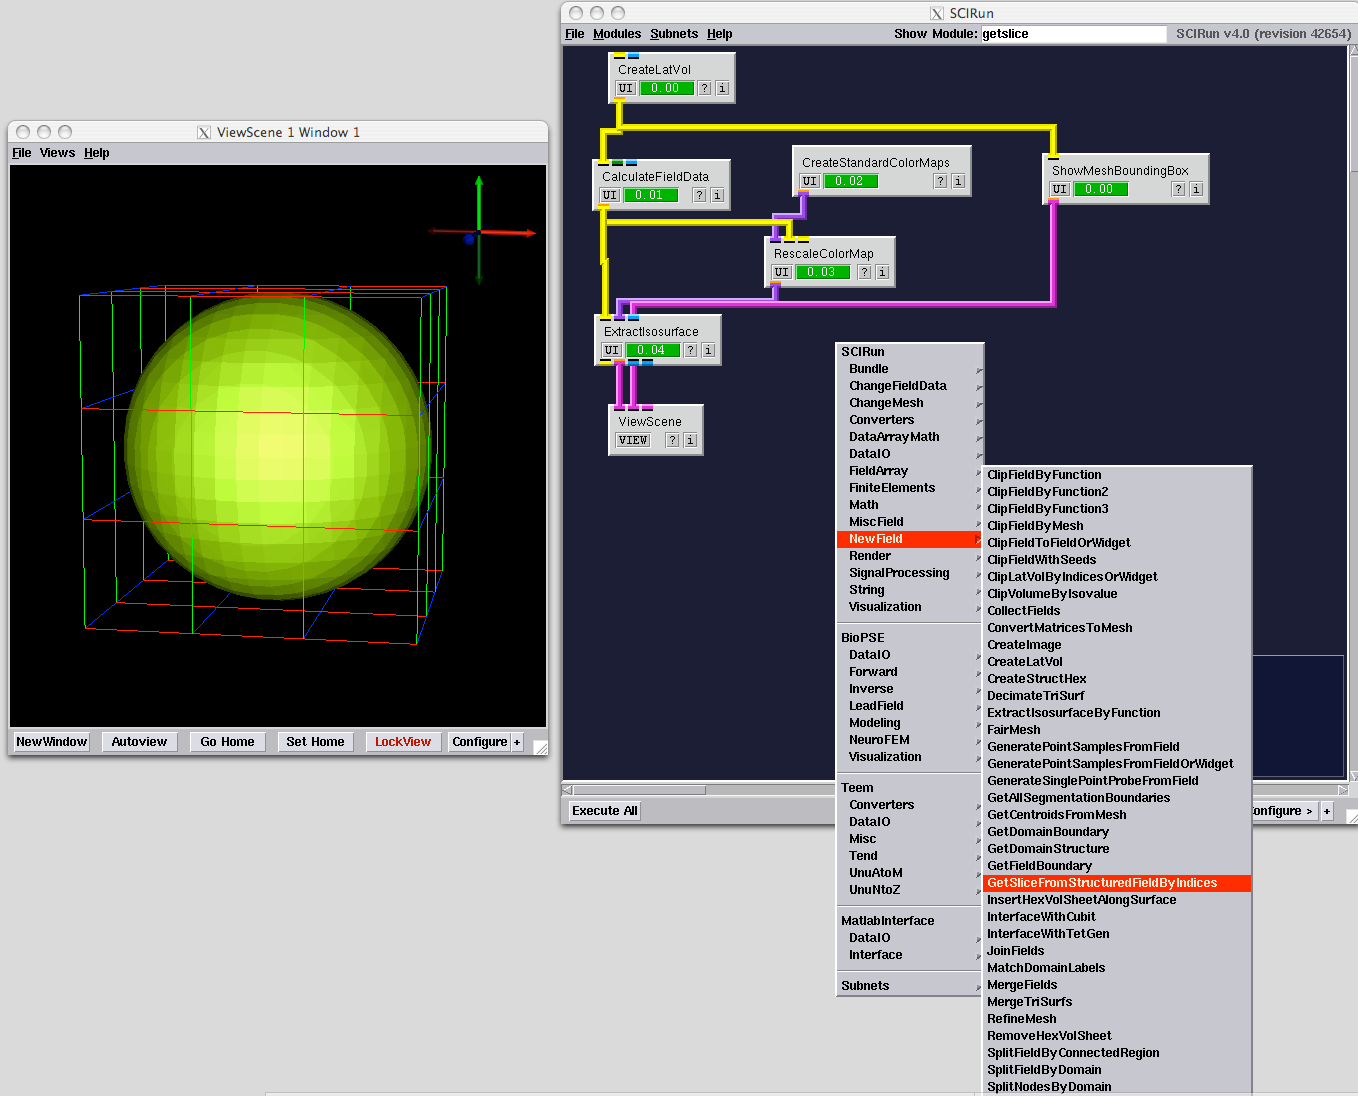
\includegraphics{BasicTutorial_figures/getslicemodule2.png}}
\caption{Using the SCIRun Network Editor's popup menu to instantiate GetSliceFromStructuredFieldByIndices.}
\label{fig:slicemod2}
\end{figure}

\begin{figure}[H]
\scalebox{0.3}{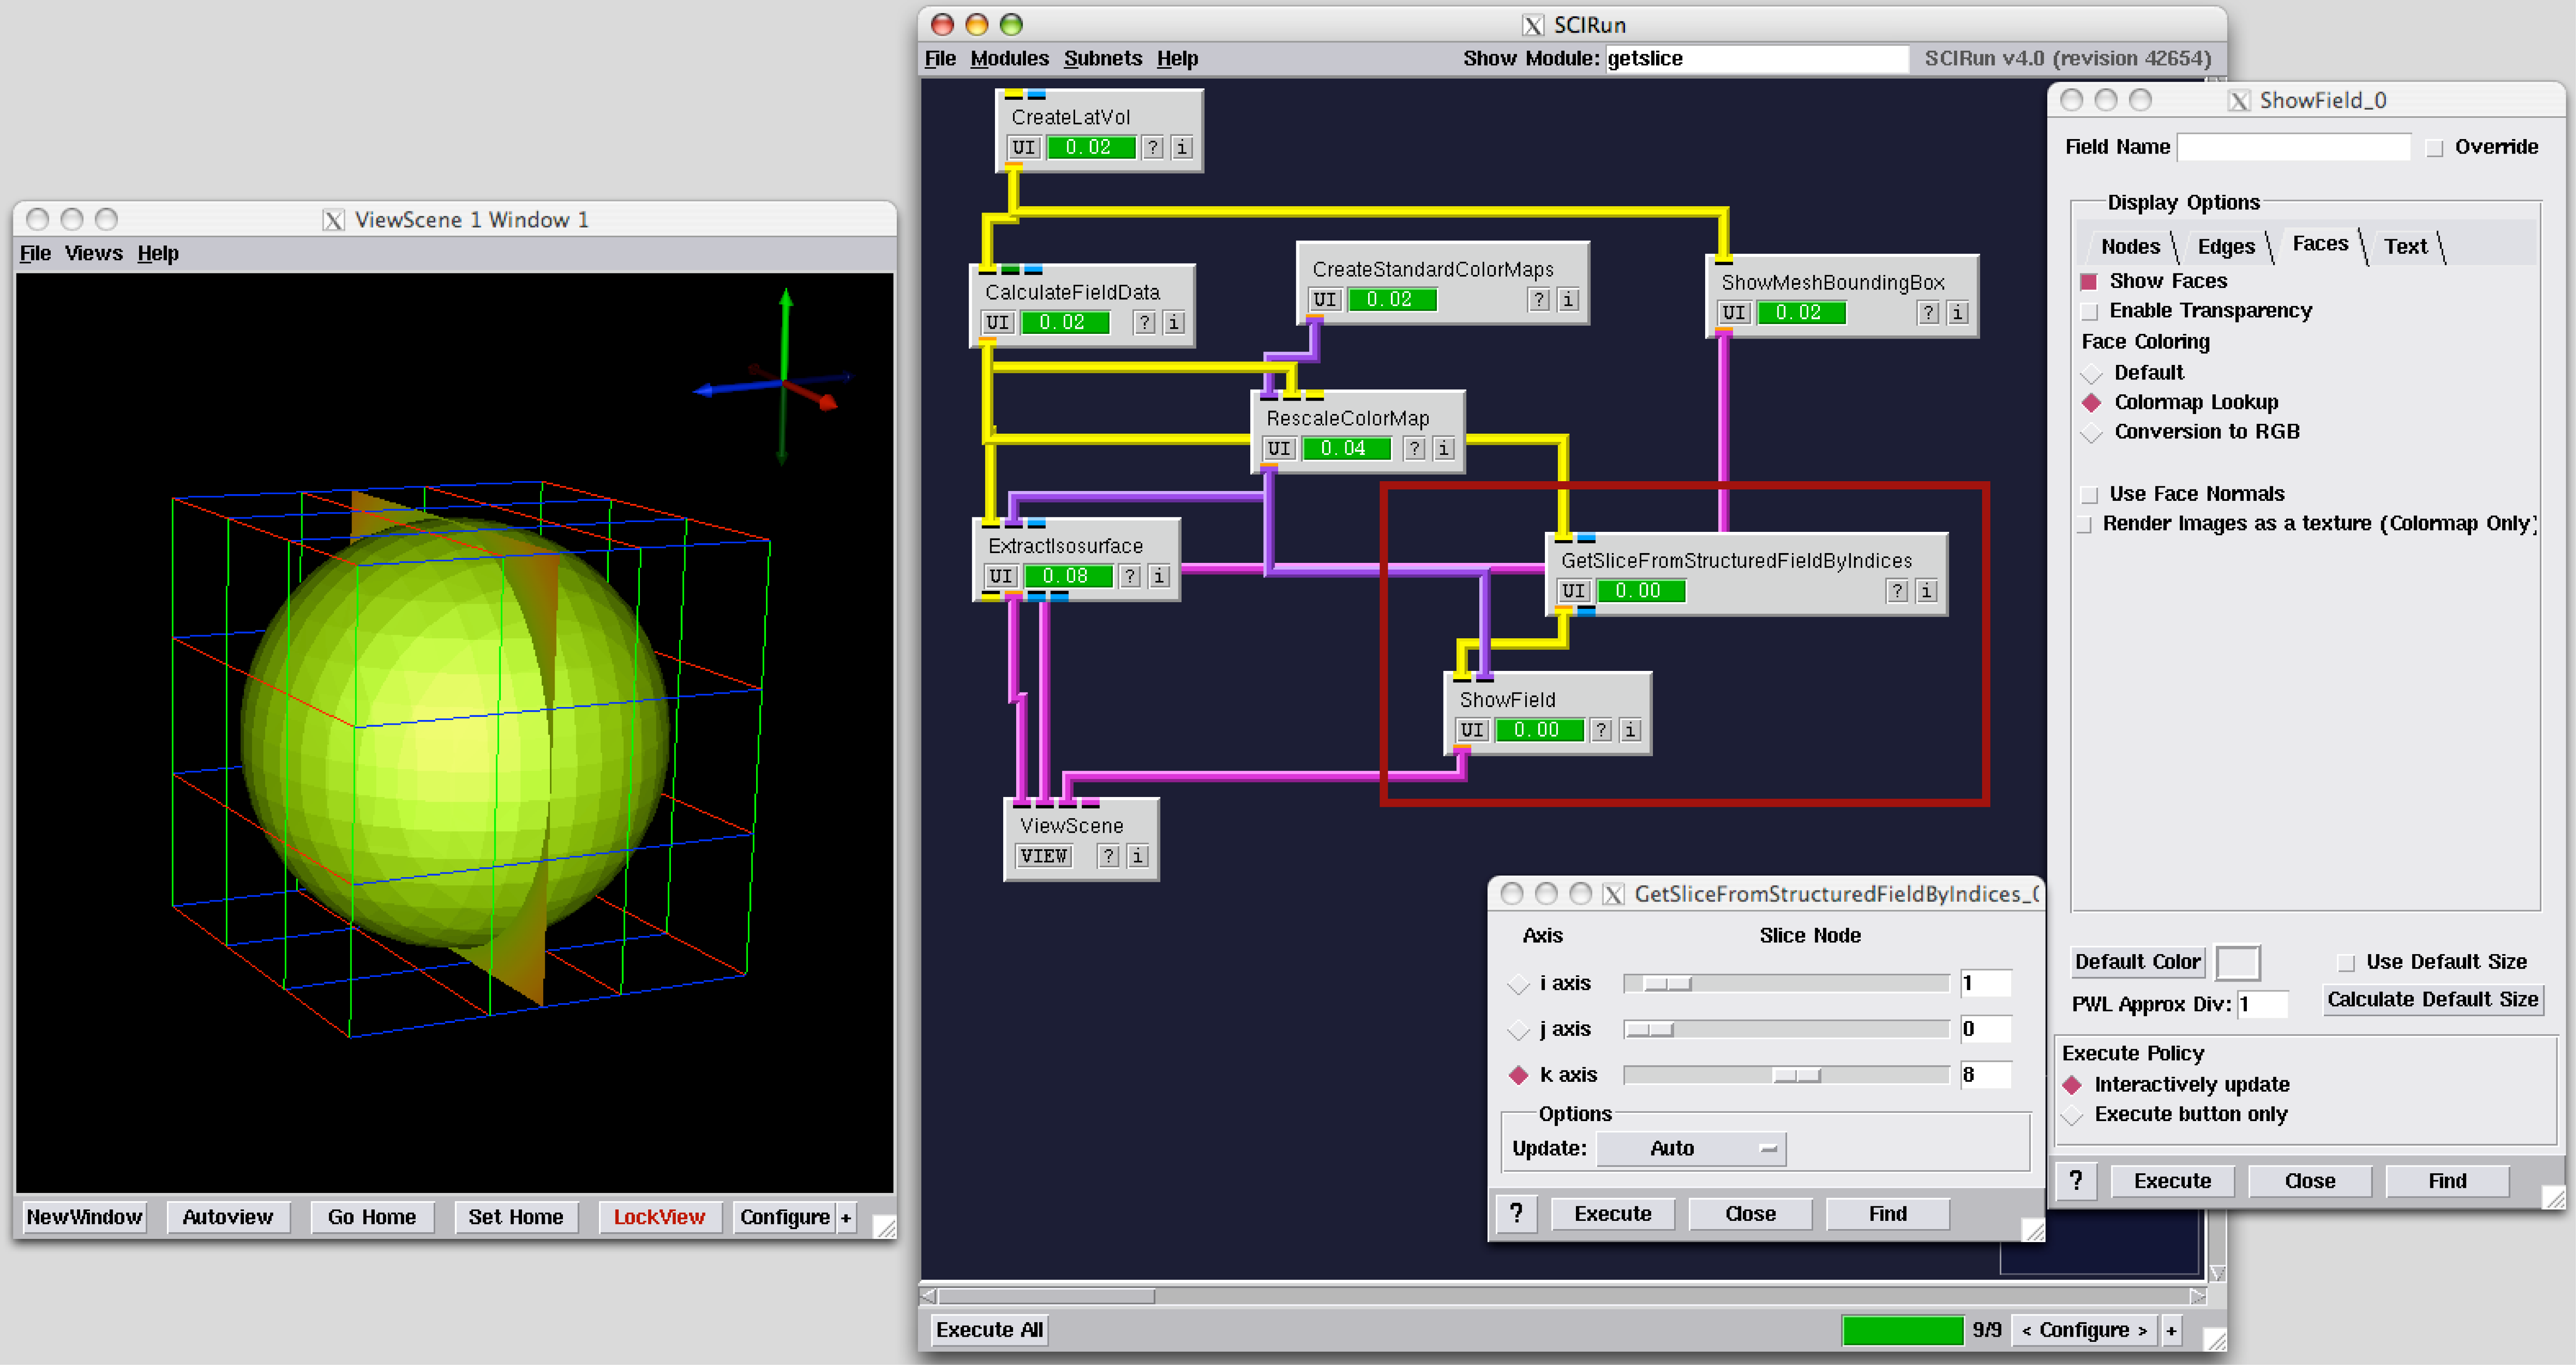
\includegraphics{BasicTutorial_figures/showfield_slice.png}}
\caption{Use ShowField to visualize the slice field.}
\label{fig:showslice}
\end{figure}

\section{Clip Field}\label{clipfieldfunc}

Clip out a subset of the original field by converting the lattice volume to an unstructured mesh using \textbf{ConvertMeshToUnstructuredMesh} (figure \ref{fig:convertmesh}) and adding \textbf{ClipFieldByFunction} (figure \ref{fig:clipfield}) to the network.
%% TODO: should highlight in image
Set the clipping location setting in ClipFieldByFunction to \emph{all nodes}.
Use the expression $DATA > 1 \&\& X < 0$ to clip the field.

\begin{figure}[H]
\scalebox{0.3}{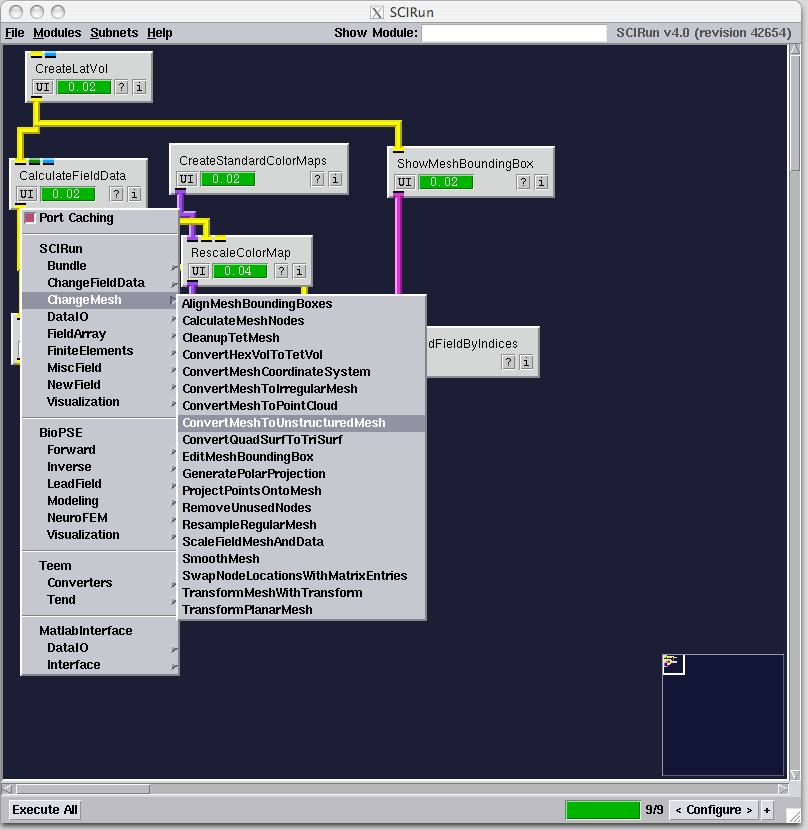
\includegraphics{BasicTutorial_figures/convertmesh.png}}
\caption{Convert the original field to an unstructured mesh.}
\label{fig:convertmesh}
\end{figure}

\begin{figure}[H]
\scalebox{0.3}{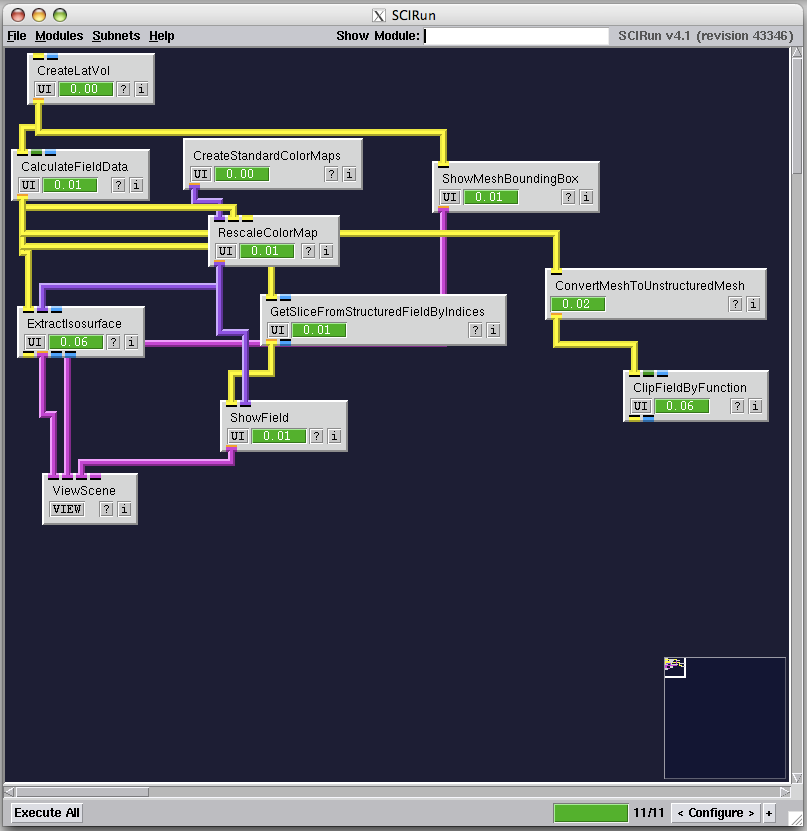
\includegraphics{BasicTutorial_figures/clipfield.png}}
\caption{Clip field.}
\label{fig:clipfield}
\end{figure}

\subsection{Extract Boundary}\label{clipvol}

Use GetFieldBoundary to extract the boundary surface from the lattice volume.
At this point, it will be necessary to map the fields by interpolating the the boundary surface field to the clipping field.
First, use \textbf{BuildMappingMatrix} to build a matrix that maps a linear combination of data values in the clipping field to a value in the boundary field. Then use \textbf{ApplyMappingMatrix} to multiply the data vector of the clipping field with the mapping matrix to obtain the data vector for the boundary surface field.

\begin{figure}[H]
\scalebox{0.3}{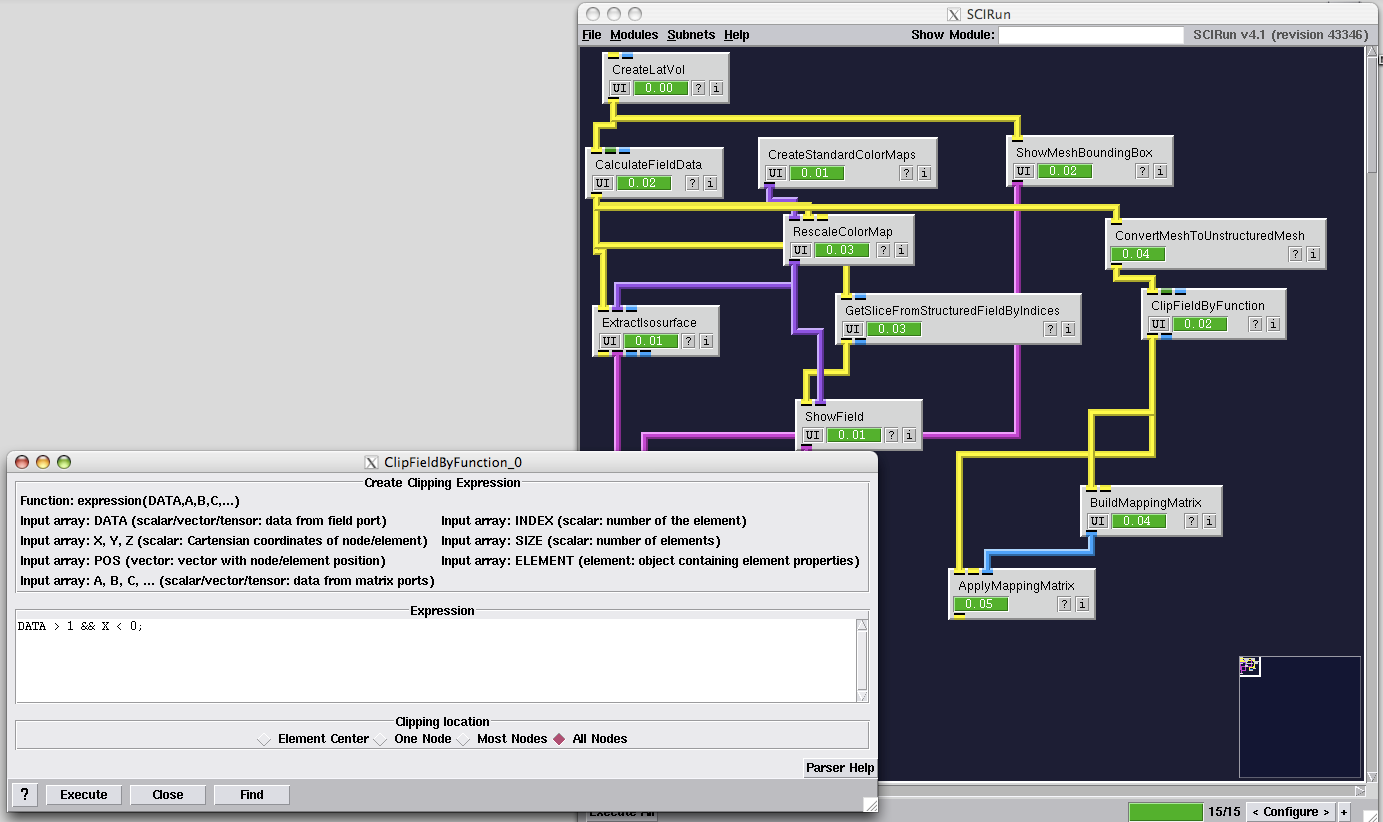
\includegraphics{BasicTutorial_figures/applymappingmatrix.png}}
\caption{Build and apply mapping.}
\label{fig:mappingmatrix}
\end{figure}

\begin{figure}[H]
\scalebox{0.3}{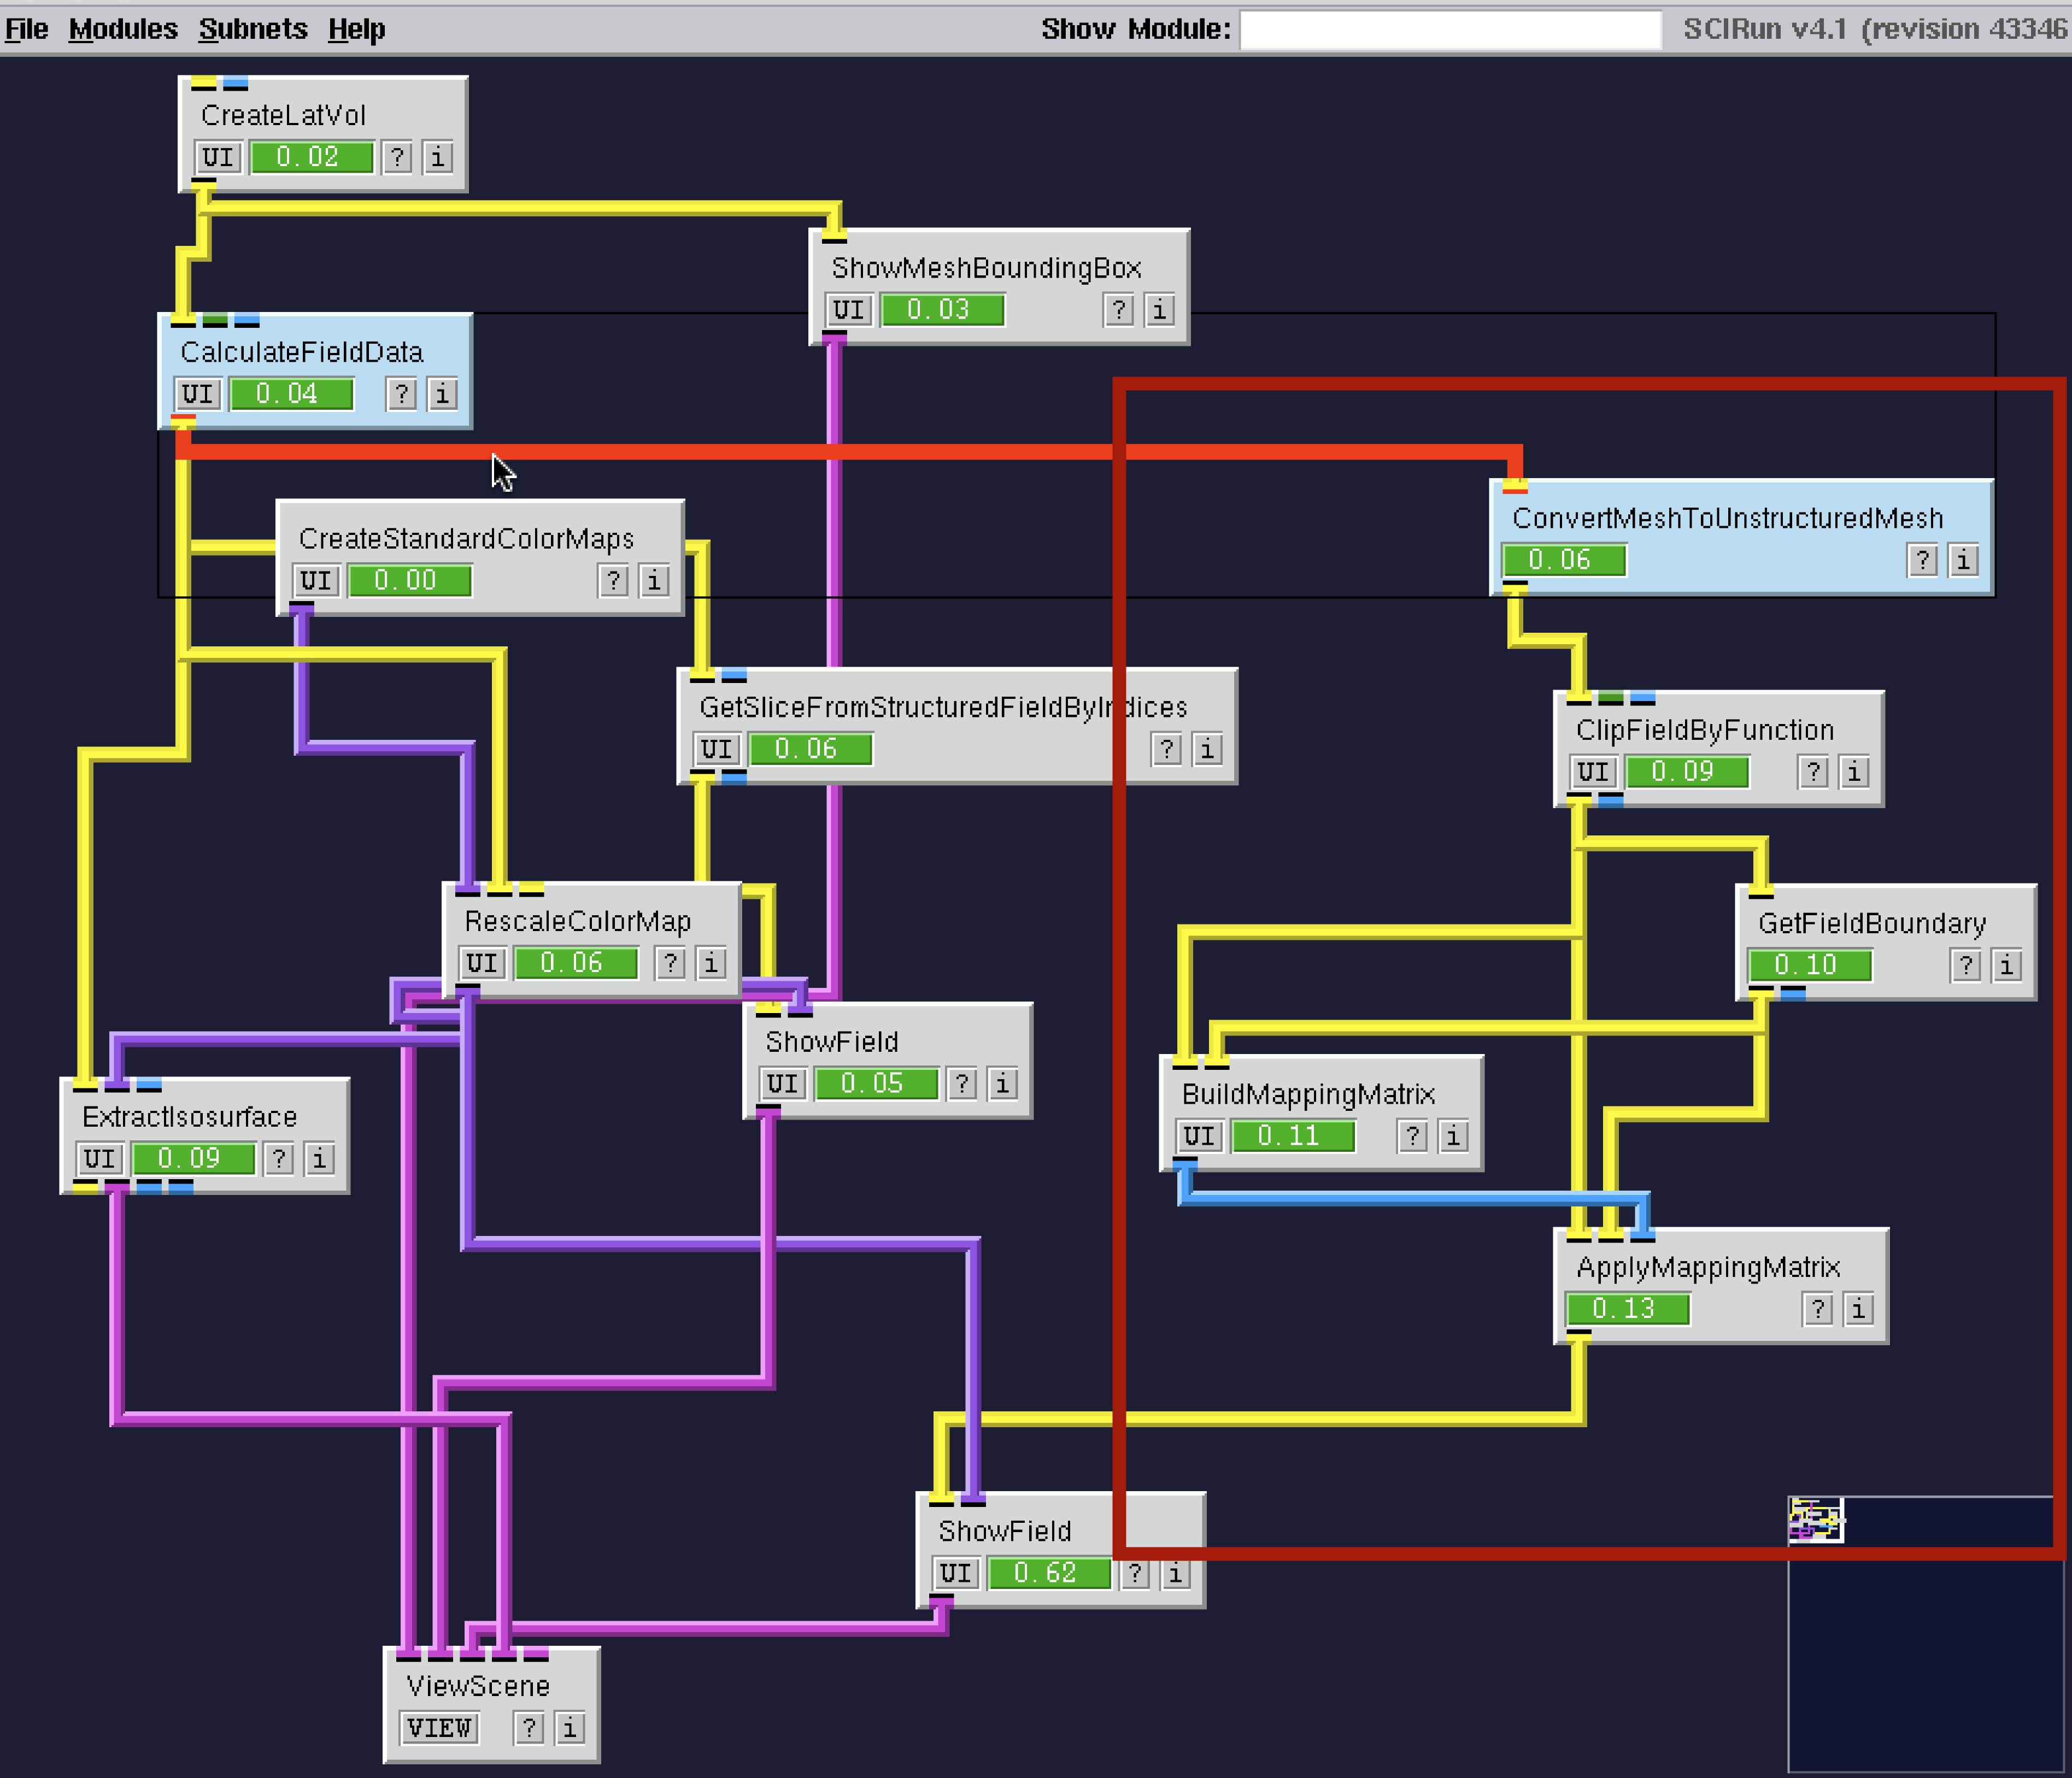
\includegraphics{BasicTutorial_figures/highlight_modules.png}}
\caption{Add mapping matrix to network.}
\label{fig:highlightmods}
\end{figure}

\begin{figure}[H]
\scalebox{0.3}{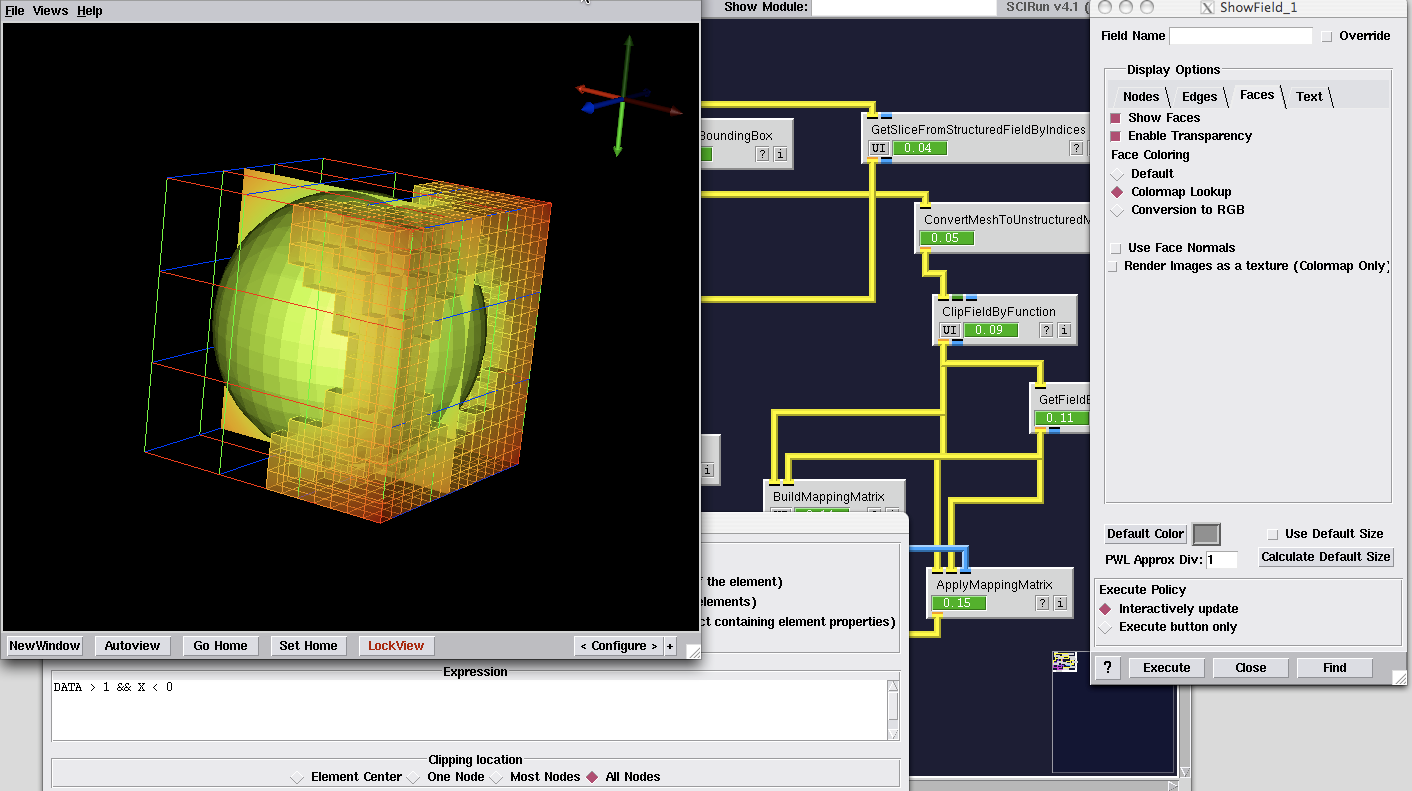
\includegraphics{BasicTutorial_figures/view_boundary.png}}
\caption{Visualize field and boundary.}
\label{fig:viewbound}
\end{figure}

Finally, it is not strictly necessary to explicitly convert the original mesh to an unstructured mesh using ConvertMeshToUnstructuredMesh because ClipFieldByFunction can implicitly convert structured mesh types to unstructured mesh types before clipping the field.
As a final exercise, delete ConvertMeshToUnstructuredMesh from the network and try to obtain the same result.

\end{document}
